\documentclass[11pt]{article}
\usepackage[margin=1in]{geometry}
\usepackage{amsmath,amssymb,amsthm,amsfonts,bm}
\usepackage{graphicx}
\usepackage{algorithm}
\usepackage{algpseudocode}
\usepackage{tikz}
\usepackage{subcaption}
\usetikzlibrary{arrows.meta,positioning,shapes.geometric,fit,calc,decorations.pathreplacing}
\usepackage[round,authoryear]{natbib}
\usepackage[colorlinks=true,linkcolor=blue,citecolor=blue,urlcolor=blue]{hyperref}
\usepackage{setspace}
\setstretch{1.1}

\newtheorem{theorem}{Theorem}
\newtheorem{lemma}{Lemma}
\newtheorem{proposition}{Proposition}
\newtheorem{corollary}{Corollary}
\theoremstyle{definition}
\newtheorem{definition}{Definition}
\theoremstyle{remark}
\newtheorem{remark}{Remark}
% restated statements in the appendix
\newenvironment{repeattheorem}[1][]{\par\medskip\noindent\textbf{#1.}\ \itshape}{\par\medskip}
\newenvironment{repeatlemma}[1][]{\par\medskip\noindent\textbf{#1.}\ \itshape}{\par\medskip}
\newenvironment{repeatproposition}[1][]{\par\medskip\noindent\textbf{#1.}\ \itshape}{\par\medskip}
\newenvironment{repeatremark}[1][]{\par\medskip\noindent\textbf{#1.}\ \itshape}{\par\medskip}
\newcommand{\up}{\rule{0pt}{2.6ex}}
\newcommand{\down}{\rule[-1.2ex]{0pt}{0pt}}
\newcommand{\Rspread}{R}
\newcommand{\FF}{F}

\title{Adaptive Influence Minimization via Deferred Frontier Blocking}
\author{Quang-Vinh Dang\\ British University Vietnam, Hung Yen, Vietnam\\ \texttt{vinh.dq4@buv.edu.vn}\\ ORCID: 0000-0002-3877-8024}
\date{}
\begin{document}
\maketitle
\begin{abstract}
Blocking the spread of a rumor or epidemic that has already started, by removing a few nodes under a fixed budget, is usually posed as a one-shot decision made before the outbreak is observed. We ask whether spending the budget gradually, as the cascade unfolds, can be worse than spending it at once, and how large the benefit can be. We introduce DEFER, a wrapper that turns any one-shot influence minimization planner into an adaptive one by re-planning every round and blocking a planned node only once the cascade has reached its neighborhood. We prove that its pure-deferral variant is never worse in expectation than the planner it wraps, up to a selection-bias caveat that we state; that a local push-down rule for early commitment is myopically optimal but can fail when several deferred targets compete for the budget; and that the adaptivity gap of influence minimization is unbounded. Experiments give a consistent picture. On star-of-paths instances, the family used in the proof, DEFER saves 0.36 to 0.97 of the spread and beats greedy, re-planning and integer-programming policies in all 18 settings. On 45 synthetic settings it is significantly better than greedy in 9 and never significantly worse, with the gains in large-cascade regimes. On small and SNAP-scale networks the differences are small, re-planning with immediate commitment is often as good, and exact integer programs did not beat greedy while running orders of magnitude slower.
\end{abstract}
\noindent\textbf{Keywords:} influence minimization; adaptive optimization; misinformation blocking; adaptivity gap

\section{Introduction}\label{sec:intro}

Consider a platform moderator who learns that a false rumor has started spreading from a handful of accounts, or a health authority that has detected a few cases of an infectious disease. Each can suspend a small number of accounts, or quarantine a small number of people, but not many. The standard operations-research treatment asks which targets to pick \emph{now}, and commits the whole budget before anything further is known. Real interventions rarely work this way: within hours or days the moderator sees which accounts the rumor has actually reached, and the authority sees which contacts have actually become infected. The practical question is whether it is better to spend the budget at once or to hold part of it back and spend it where the outbreak actually goes. Holding back is risky, because a cascade can pass through a node before it is blocked, but it also avoids spending budget on targets the cascade never reaches. This paper quantifies that trade-off.

The problem is \emph{influence minimization} (IMIN) \citep{xie2023,xie2024}: given the seeds of a cascade under the independent cascade model and a budget of vertices that can be removed, choose the vertices that minimize the expected final spread. IMIN is the natural complement of influence \emph{maximization} \citep{kempe2003}. Unlike maximization its objective is not supermodular, so greedy selection carries no approximation guarantee, and the problem is NP-hard and hard to approximate \citep{xie2023}. Every published IMIN algorithm, including AdvancedGreedy and GreedyReplace \citep{xie2023,xie2024} and the Sandwich family \citep{wang2024sandwich}, is \emph{one-shot}: the entire budget is spent before the cascade is observed.

\paragraph{What we ask.} Two questions follow, and neither has, to our knowledge, been answered formally for IMIN. Can adapting to the unfolding cascade ever hurt, relative to a one-shot plan? And how large can the benefit of adapting be? A third question is practical: in which networks and regimes does adapting actually pay, and is it worth the added computation compared with solving the one-shot problem exactly?

\paragraph{What we find.} Table~\ref{tab:summary} gives the answers in one place, with the sections where each is established.

\begin{table}[h]
\centering
\caption{Summary of results.}\label{tab:summary}
\small
\begin{tabular}{@{}p{0.26\textwidth}p{0.55\textwidth}p{0.11\textwidth}@{}}
\hline
\up Question & Answer & Where \\
\hline
\up Can adapting hurt? & Pure deferral (\texttt{DEFER-nopush}) is never worse in expectation than the planner it wraps, up to a selection-bias caveat. Early commitment by the push-down rule is optimal for a single target but can make DEFER worse than its planner when targets compete for the budget. & Sec.~\ref{sec:defer-theory} \\
How large can the benefit be? & Unbounded. On the star-of-paths family the saving ratio approaches $(1-(1-p)^\Delta)/p$ and the spread ratio grows without limit. In simulation DEFER saves $0.36$--$0.97$ of the spread there and exceeds the best of AG, GR, COMMIT and the one-shot ILP by at least $0.27$ in all 18 settings. & Sec.~\ref{sec:defer-theory}, \ref{sec:exp-sop} \\
Where does it help in practice? & In large-cascade regimes. Over 45 synthetic settings DEFER is significantly better than AG in 9, better than COMMIT in 6, and never significantly worse. On small and SNAP-scale networks the gains are small ($0.2$--$1.9$ percentage points at budget $20$ on four SNAP-scale networks). & Sec.~\ref{sec:exp-regime}, \ref{sec:defer-experiments} \\
Does exact optimization remove the need? & No. A time-indexed scenario ILP, one-shot or staged, did not beat greedy (within $0.02$ of AG in 13 of 19 cells) and ran far slower; the ILP as DEFER's planner matched the ILP alone. & Sec.~\ref{sec:exp-ilp} \\
What does it cost? & DEFER's cost is AG's per-round cost times the number of rounds, about $2.5$--$7\times$ AG's wall-clock time. & Sec.~\ref{sec:defer-theory}, \ref{sec:complexity-comparison} \\
\hline
\end{tabular}
\end{table}

\paragraph{Contributions.} (i) DEFER, a wrapper that makes any one-shot planner adaptive (Section~\ref{sec:defer}). (ii) Three theoretical results on when adapting is safe and how much it can help: weak dominance of pure deferral, a local optimality result for push-down together with a counterexample showing it does not extend, and an unbounded adaptivity gap with an explicit construction (Section~\ref{sec:defer-theory}). (iii) An empirical study designed to show where the theory bites: the proof's own family, a grid of synthetic regimes with paired comparisons, empirical networks, and exact integer-programming baselines (Section~\ref{sec:experiments}). The study reports the settings in which DEFER does not help as well as those in which it does.

\paragraph{Roadmap.} Section~\ref{sec:related} reviews related work and Section~\ref{sec:prelim} fixes the model. Section~\ref{sec:defer} presents DEFER, first the algorithm, then a worked example that shows the effect in numbers, then the guarantees, each preceded by a plain-language statement of what it says. Section~\ref{sec:experiments} reports the experiments and Section~\ref{sec:discussion} discusses them and the limitations. Proofs and further details are in the appendices.

\section{Related Work}\label{sec:related}

\textbf{Influence minimization.} \citet{xie2023} introduce IMIN, prove NP-hardness and inapproximability, and give AdvancedGreedy. \citet{xie2024} extend this with GreedyReplace. The Sandwich lower/upper-bound family we use as the LSBM baseline is due to \citet{wang2024sandwich}.

\textbf{Rumor and misinformation blocking before IMIN.} Limiting an already-spreading process's damage by removing or countering a small vertex set predates IMIN's formal treatment: \citet{budak2011} counter-seed a rival campaign under independent cascade; \citet{he2012} extend this to competitive linear threshold; \citet{nguyen2012} and \citet{wang2013blocking} study node and edge removal directly; \citet{fan2013} add a removal-cost budget; \citet{wang2016drimux} and \citet{tong2018} treat dynamic and multi-campaign settings; \citet{farajtabar2017} model the cascade as a Hawkes process steered by reinforcement learning; \citet{yan2020} study blocker placement under a fixed budget; and \citet{zareie2021} survey this line. \citet{xiang2024} is a recent pertinence-constrained variant. None of this line treats commitment timing as a decision variable.

\textbf{Exact and optimization-based methods.} Influence minimization and related blocking problems have also been attacked with exact mathematical-programming methods, which matter for the dynamic setting studied here. \citet{taninmis2022} give an improved $x$-space algorithm for min--max bilevel problems, with misinformation spread in social networks as an application, and \citet{taninmis2024} develop Benders decomposition algorithms for minimizing the spread of harmful contagions. We are not aware that either treats the timing of commitment as a decision, but a time-indexed formulation extends naturally to staged budgets: the blocking variables carry a time index, the budget constraint couples the stages, and a node cannot be blocked after the cascade has reached it. Section~\ref{sec:exp-ilp} implements such a formulation and benchmarks it. We did not implement the cut-based Benders or bilevel algorithms themselves.

\textbf{Adaptive and sequential decision problems.} Adaptive variants of influence \emph{maximization} are well studied: \citet{golovinkrause2011} give the adaptive-submodularity framework; \citet{seemansinger2013} apply two-stage adaptive seeding; and \citet{tong2017} give an adaptive maximization algorithm that re-plans as the network changes, structurally similar to DEFER but for the maximization objective. For stochastic monotone submodular maximization, the adaptivity gap, introduced by \citet{deangoemansvondrak2008} for stochastic knapsack, is bounded by a constant \citep{asadpournazerzadeh2016}. Theorem~\ref{thm:adaptivity-gap} shows the opposite for IMIN, an unbounded gap, attributable to the lack of supermodularity of $\FF$ \citep{xie2023}. To our knowledge no prior work formalizes an adaptive variant of IMIN or proves results of the shape of Lemma~\ref{lem:defer-free} or Theorem~\ref{thm:adaptivity-gap} for this minimization problem.

\section{Preliminaries}\label{sec:prelim}
\subsection{The independent cascade model}\label{sec:ic-model}

$G=(V,E)$ is a directed graph,
$n=|V|$, $m=|E|$, with edge probabilities $p:E\to(0,1]$. A live-edge
realization $\omega\in\{0,1\}^E$ is drawn with
$\Pr[\omega]=\prod_{e}p_e^{\omega_e}(1-p_e)^{1-\omega_e}$. For a seed set
$S\subseteq V$ and blocked set $B\subseteq V\setminus S$, write
$G_B=G[V\setminus B]$ and let $\Rspread(\omega,B)\subseteq V\setminus B$ be
the set of vertices reachable from $S$ using only live edges of $G_B$. The
\emph{expected spread} is
\begin{equation}\label{eq:spread}
\FF(B)\;=\;\mathbb E_\omega\bigl[\,|\Rspread(\omega,B)\setminus S|\,\bigr].
\end{equation}

\subsection{Problem formalization}\label{sec:formalization}

\begin{definition}[IMIN, one-shot]\label{def:imin}
Given $G$, $p$, seed set $S$, and budget $b\in\mathbb N$, the
\emph{influence minimization} (IMIN) problem is
\begin{equation}\label{eq:imin}
\min_{B\subseteq V\setminus S}\ \FF(B)
\qquad\text{subject to}\qquad
|B|\le b.
\end{equation}
\end{definition}

\noindent \citet{xie2023} show Problem~\eqref{eq:imin} is NP-hard and hard
to approximate within any constant factor unless P$=$NP, and that $\FF$ is
not supermodular in $B$ under the IC model, so the greedy
$(1-1/e)$-guarantee available for influence \emph{maximization}
\citep{kempe2003} does not transfer.

To formalize the adaptive variant, let a \emph{history} up to round $t$ be
$h_t=(N_0,N_1,\dots,N_t)$, the sequence of newly activated sets observed so
far (full-adoption feedback: which vertices activate each round, not which
live edges carried the activation). Let $\mathcal H$ denote the set of all
histories of any length.

\begin{definition}[Adaptive policy]\label{def:policy}
An \emph{adaptive blocking policy} is a function
$\pi:\mathcal H\to 2^V$ mapping each history $h_t$ to a set of
not-yet-activated, not-yet-blocked vertices to additionally block in round
$t+1$, subject to $\sum_{t}|\pi(h_t)|\le b$ over the run of the cascade.
Write $\sigma(\pi)$ for the (random) final spread beyond $S$ that results
from running the cascade under policy $\pi$.
\end{definition}

\begin{definition}[IMIN, adaptive]\label{def:adaptive-imin}
Given $G$, $p$, $S$, and budget $b$, the \emph{adaptive} IMIN problem is
\begin{equation}\label{eq:adaptive-imin}
\min_{\pi}\ \mathbb E\bigl[\sigma(\pi)\bigr]
\qquad\text{subject to}\qquad
\textstyle\sum_t|\pi(h_t)|\le b\ \text{a.s.}
\end{equation}
A one-shot policy is the special case $\pi(h_0)=B$ for a fixed
$B$ with $|B|\le b$ and $\pi(h_t)=\varnothing$ for $t\ge1$, so
Problem~\eqref{eq:imin} is exactly Problem~\eqref{eq:adaptive-imin}
restricted to one-shot policies, and
$\min_\pi\mathbb E[\sigma(\pi)]\le\min_{|B|\le b}\FF(B)$ trivially, since
every one-shot policy is a feasible (adaptive) policy. The
\emph{adaptivity gap} of an instance is the ratio of the right-hand side to
the left-hand side of this inequality; Theorem~\ref{thm:adaptivity-gap}
shows this gap is unbounded.
\end{definition}

DEFER (Section~\ref{sec:defer}) is a construction of a specific policy $\pi_{\mathrm{DEFER}}$, parameterized by a choice of one-shot planner $\mathcal P$, that is feasible for Problem~\eqref{eq:adaptive-imin} and provably no worse than $\mathcal P$'s own one-shot value in its pure-deferral form (Theorem~\ref{thm:defer-dominates}). Table~\ref{tab:notation} lists the notation.

\begin{table}[h]
\centering
\caption{Notation.}\label{tab:notation}
\small
\begin{tabular}{@{}ll@{}}
\hline
\up Symbol & Meaning \\
\hline
\up $G=(V,E)$, $n$, $m$ & graph, vertex count, edge count \\
$p:E\to(0,1]$ & independent-cascade edge probabilities \\
$S$, $B$, $b$ & seed set, blocked set, blocking budget \\
$\omega$, $\Rspread(\omega,B)$ & live-edge realization, reachable set under $\omega$ with $B$ removed \\
$\FF(B)$ & expected spread with blocking set $B$ (Eq.~\ref{eq:spread}) \\
$F_t$, $A_t$, $N_t$ & round-$t$ frontier, active set, newly activated set \\
$P_t$, $L$, $C_t$ & round-$t$ plan, uncommitted leftover, vertices committed this round \\
$q_v$, $c_v$, $\lambda_t$ & exposure probability, child count, shadow price of a budget unit \\
\down $\mathcal P$ & one-shot planner wrapped by DEFER \\
\hline
\end{tabular}
\end{table}
\section{DEFER: Adaptive Influence Minimization by Deferred Frontier Blocking}\label{sec:defer}

\subsection{Algorithm}\label{sec:defer-algo}

DEFER wraps a one-shot planner $\mathcal P$ (any IMIN algorithm; by default
a dominator-tree greedy planner with isolation moves). At each round it
re-plans on the currently reachable region, keeps whichever of the new plan
and the previous round's uncommitted leftover looks better on freshly drawn
samples (\emph{plan protection}), and commits only the fraction of the plan
that is both exposed to the current frontier and passes a push-down test.

\begin{algorithm}[h]
\caption{DEFER}\label{alg:defer}
\begin{algorithmic}[1]
\Require graph $G$, probabilities $p$, seeds $S$, budget $b$, sample size
  $\theta$, one-shot planner $\mathcal P$
\State $A_0\gets S$, $B_0\gets\varnothing$, $F_0\gets S$, $L\gets\varnothing$ (uncommitted leftover)
\For{$t=0,1,2,\dots$ while the cascade is alive and $|B_t|<b$}
  \State $b_t\gets b-|B_t|$
  \State draw $\theta$ live-edge subgraphs reachable from $F_t$ avoiding $A_t\cup B_t$
  \State $P'\gets\mathcal P(\text{seeds}=F_t,\ \text{forbidden}=A_t\cup B_t,\ \text{budget}=b_t)$ on the samples
  \State draw a fresh, held-out set of $\theta$ live-edge subgraphs (disjoint from those used to compute $P'$)
  \State $\hat d\gets$ sample-average saving of $P'$ minus sample-average saving of $L$ on the held-out draws; $\widehat{\mathrm{se}}\gets$ their standard error
  \If{$\hat d>\widehat{\mathrm{se}}$} \Comment{plan protection: swap only if the improvement exceeds one held-out standard error}
    \State $P_t\gets P'$
  \Else
    \State $P_t\gets L$
  \EndIf
  \State $X_t\gets$ inactive, unblocked out-neighbors of $F_t$
  \State $\lambda_t\gets$ smallest marginal saving among the picks of $P_t$ (0 if $P_t$ does not exhaust $b_t$)
  \For{$v\in P_t\cap X_t$}\label{alg:pushdown-start}
    \State $q_v\gets 1-\prod_{u\in F_t}(1-p(u,v))$; $c_v\gets$ inactive unblocked out-degree of $v$
    \If{$\lambda_t=0$ \textbf{or} $q_v\,(c_v+1/\lambda_t)\ge 1$} \Comment{push-down rule, Lemma~\ref{lem:pushdown} (myopic, no budget-contention guarantee -- Remark~\ref{rem:pushdown-counterexample})}
      \State block $v$ now
    \EndIf
  \EndFor\label{alg:pushdown-end}
  \State $L\gets P_t\setminus(\text{blocked this round})$
  \State observe $N_{t+1}$; update $A_{t+1},F_{t+1}$
\EndFor
\end{algorithmic}
\end{algorithm}

The push-down rule compares spending one budget unit on an exposed node $v$
now against waiting one round and, if $v$ activates (probability $q_v$),
protecting its $c_v$ children instead while losing $v$ itself. When the
planner is deterministic given the samples and no new information arrives,
DEFER reduces to lazily committing the one-shot planner's own plan
(Lemma~\ref{lem:defer-free}); the two ablations used in
Section~\ref{sec:experiments} are COMMIT (same loop, but the whole plan is
committed every round) and the one-shot planners run without any wrapper.
Figure~\ref{fig:defer-flow} shows the round-by-round control flow this
paragraph and Algorithm~\ref{alg:defer} describe.

\begin{figure}[h]
\centering
\begin{subfigure}[t]{0.32\textwidth}
\centering
\resizebox{\linewidth}{!}{%
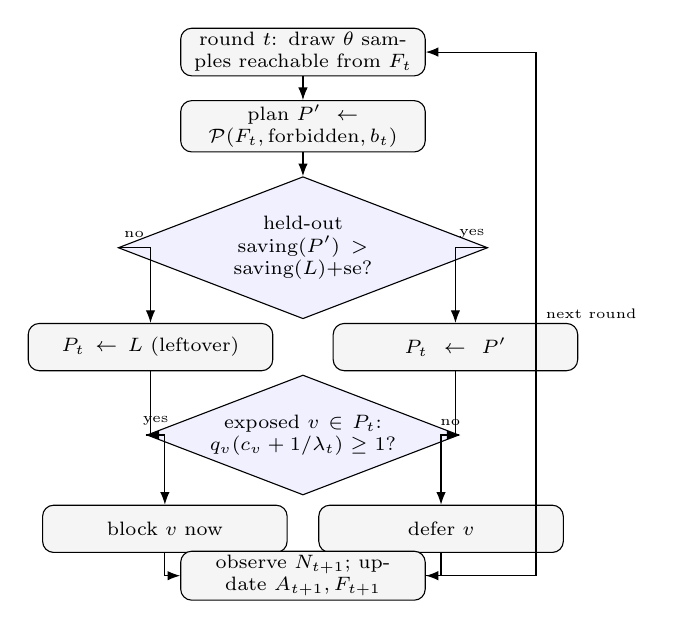
\begin{tikzpicture}[
  node distance=3mm and 8mm,
  box/.style={draw, rounded corners, align=center, fill=gray!8, font=\scriptsize, text width=30mm, minimum height=6mm, inner sep=1.5pt},
  dec/.style={draw, diamond, aspect=2.6, align=center, fill=blue!6, font=\scriptsize, text width=25mm, inner sep=0.5pt},
  arr/.style={-{Latex[length=1.6mm]}}
]
\node[box] (draw) {round $t$: draw $\theta$ samples reachable from $F_t$};
\node[box, below=of draw] (plan) {plan $P'\gets\mathcal P(F_t,\text{forbidden},b_t)$};
\node[dec, below=of plan] (protect) {held-out saving$(P')>$ saving$(L)+$se?};
\node[box, below left=5mm and -8mm of protect] (keepold) {$P_t\gets L$ (leftover)};
\node[box, below right=5mm and -8mm of protect] (keepnew) {$P_t\gets P'$};
\node[dec, below=7mm of protect] (push) {exposed $v\in P_t$: $q_v(c_v+1/\lambda_t)\ge1$?};
\node[box, below left=5mm and -8mm of push] (commitnow) {block $v$ now};
\node[box, below right=5mm and -8mm of push] (defer) {defer $v$};
\node[box, below=7mm of push] (obs) {observe $N_{t+1}$; update $A_{t+1},F_{t+1}$};
\draw[arr] (draw) -- (plan);
\draw[arr] (plan) -- (protect);
\draw[arr] (protect) -| node[near start, above, font=\tiny]{no} (keepold);
\draw[arr] (protect) -| node[near start, above, font=\tiny]{yes} (keepnew);
\draw[arr] (keepold) |- (push);
\draw[arr] (keepnew) |- (push);
\draw[arr] (push) -| node[near start, above, font=\tiny]{yes} (commitnow);
\draw[arr] (push) -| node[near start, above, font=\tiny]{no} (defer);
\draw[arr] (commitnow) |- (obs);
\draw[arr] (defer) |- (obs);
\draw[arr] (obs.east) -- ++(14mm,0) |- node[pos=0.25, right, font=\tiny]{next round} (draw.east);
\end{tikzpicture}}
\caption{DEFER's per-round control flow}
\label{fig:defer-flow}
\end{subfigure}%
\hfill
\begin{subfigure}[t]{0.64\textwidth}
\centering
\resizebox{\linewidth}{!}{%
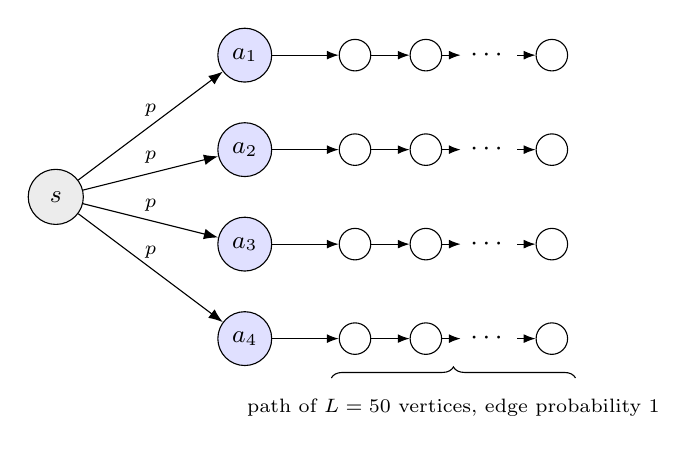
\begin{tikzpicture}[
  seed/.style={draw, circle, fill=gray!15, minimum size=7mm, font=\small},
  gw/.style={draw, circle, fill=blue!12, minimum size=6mm, font=\small},
  pv/.style={draw, circle, fill=white, minimum size=4mm, font=\scriptsize},
  edgelab/.style={font=\scriptsize, above}
]
\node[seed] (s) at (0,0) {$s$};
\foreach \i/\y in {1/1.8,2/0.6,3/-0.6,4/-1.8} {
  \node[gw] (a\i) at (2.4,\y) {$a_{\i}$};
  \draw[-{Latex[length=1.8mm]}] (s) -- node[edgelab]{$p$} (a\i);
  \node[pv] (v\i a) at (3.8,\y) {};
  \node[pv] (v\i b) at (4.7,\y) {};
  \node (dots\i) at (5.5,\y) {$\cdots$};
  \node[pv] (v\i c) at (6.3,\y) {};
  \draw[-{Latex[length=1.5mm]}] (a\i) -- (v\i a);
  \draw[-{Latex[length=1.5mm]}] (v\i a) -- (v\i b);
  \draw[-{Latex[length=1.5mm]}] (v\i b) -- (dots\i);
  \draw[-{Latex[length=1.5mm]}] (dots\i) -- (v\i c);
}
\draw[decorate, decoration={brace, amplitude=4pt}] (3.5,-2.3) -- (6.6,-2.3)
  node[midway, below=4pt, font=\scriptsize]{path of $L=50$ vertices, edge probability $1$};
\end{tikzpicture}}
\caption{The star-of-paths instance behind Theorem~\ref{thm:adaptivity-gap}}
\label{fig:star-of-paths}
\end{subfigure}

\caption{DEFER's control flow, and the star-of-paths worked-example instance. (a) Plan protection (top decision) chooses between the new plan and the
leftover $L$ using a fresh held-out sample; push-down (bottom decision)
then decides, for each planned vertex exposed to the frontier, whether to
commit it now or defer it to a child (Lemma~\ref{lem:pushdown}). (b) Each
of the $\Delta=4$ gateways $a_i$ activates independently with probability
$p=0.1$ from seed $s$ and, if live, deterministically propagates down its
own private length-$L$ path. A one-shot policy commits before observing
which gateways activate; DEFER waits one round, observes $N_1$, and
blocks the first path vertex of one confirmed-live branch (the gateway
itself can no longer be blocked once activated).}
\end{figure}

\subsection{Worked example}\label{sec:defer-example}

Before stating the formal results of Section~\ref{sec:defer-theory}, we show
the central effect on a small instance. The idea is that a one-shot policy
must pay to protect against every threat that \emph{might} materialize,
while a deferred policy waits and pays only for threats that are seen to
materialize. The instance below is the one used later to prove that this gap
can be arbitrarily large (Theorem~\ref{thm:adaptivity-gap}); here we only
compute its numbers. It is a star-of-paths instance
(Figure~\ref{fig:star-of-paths}), with $\Delta=4$ branches,
per-branch activation probability $p=0.1$, path length $L=50$, and budget
$b=1$. Seed $s$ has four out-neighbors $a_1,\dots,a_4$, each independently
live with probability $p$; each $a_i$ that activates starts a private,
deterministic path of $L=50$ further vertices. With no intervention, each
branch contributes $L+1=51$ vertices to the spread with probability $p$,
so the expected total spread is $\Delta p(L+1)=4(0.1)(51)=20.4$.

A one-shot policy with budget 1 must pick a single vertex to remove before
observing anything; by symmetry the best it can do is remove one branch's
gateway $a_i$ outright, which pre-empts that branch's entire contribution
regardless of whether $(s,a_i)$ would have been live. Its expected spread
is then the sum over the remaining three branches,
$(\Delta-1)p(L+1)=3(0.1)(51)=15.3$.

DEFER instead waits one round. It observes $N_1=\{a_i:(s,a_i)\text{ live}\}$
-- the number of active branches $k$ is $\mathrm{Binomial}(4,0.1)$, so
$k=0$ with probability $0.656$, $k=1$ with probability $0.292$, $k=2$ with
probability $0.049$, and $k\ge3$ with probability $0.004$ -- and spends its
one block on the first path vertex of one active branch (blocking $a_i$
itself is no longer possible once it has activated). This seals that one
branch's continuation at a cost of only the vertex $a_i$ already reached,
while $k-1$ other active branches, if any, still propagate their full
length-$L$ path. DEFER's expected spread is
$\Delta p+L\cdot\mathbb E[(k-1)^+]=0.4+50(0.0561)=3.205$, using
$\mathbb E[(k-1)^+]=\sum_{k\ge1}(k-1)\Pr[k]=0.0561$ computed from the
binomial probabilities above. Theorem~\ref{thm:adaptivity-gap} makes two
separate claims about this instance, and it is worth checking both
numerically. The \emph{saving} each policy achieves relative to no
intervention is $p(L+1)=0.1(51)=5.1$ for one-shot and
$L(1-(1-p)^\Delta)=50(1-0.9^4)=17.195$ for DEFER, a ratio of
$17.195/5.1\approx3.372$ -- below the limiting bound
$(1-(1-p)^\Delta)/p\approx3.439$ by exactly the factor $L/(L+1)=50/51$ the
theorem predicts, and approaching it as $L$ grows. The ratio of the two
policies' \emph{spreads} themselves is a different quantity,
$15.3/3.205\approx4.77$ here, and it is not bounded by $3.439$ as $p$
shrinks: unlike the saving ratio, which depends only on $\Delta$ and $p$,
the spread ratio needs $L$ to grow along with $1/p$ to reach its own
$L\to\infty$ limit $2/(\Delta p)$, which is unbounded as $p\to0$ at fixed
$\Delta$ (Theorem~\ref{thm:adaptivity-gap}'s proof verifies this
numerically at $\Delta=4$, $p=0.01$, $L=5000$: spread ratio $\approx49.7$,
close to $2/(\Delta p)=50$).

The qualitative point survives far more general instances: a one-shot
policy pays for protection whether or not the threat it protects against
ever materializes, while DEFER pays only for branches actually observed
live. Push-down (Lemma~\ref{lem:pushdown}) tells DEFER \emph{when} this is
worth it -- here, $c_v=1$, $q_v=p=0.1$ is small relative to the shadow
price $\lambda\approx pL\approx5$, so $q_v(c_v+1/\lambda)<1$ holds and
every exposed branch vertex is deferred; with $q_v$ near $1$ (a
near-certain threat) the same rule commits right away instead, recovering
one-shot behavior exactly where deferring would not help.

\subsection{Theoretical guarantees}\label{sec:defer-theory}

Full proofs of every result in this section are given in
Appendix~\ref{ec:defer-proofs}. Before the formal statements, here
is what they say in plain terms.
\begin{itemize}
\item \emph{Waiting costs nothing in itself} (Lemma~\ref{lem:defer-free}):
  if the targets are fixed in advance, blocking each one only when the
  cascade reaches its doorstep gives exactly the same outcome as blocking
  all of them at time $0$, and may leave budget unspent.
\item \emph{Adapting to a better plan cannot hurt, if switching is
  disciplined} (Theorem~\ref{thm:defer-dominates}): re-planning from what
  has been observed is safe as long as a new plan replaces the old one only
  when it is clearly better on fresh data.
\item \emph{Committing an exposed target early versus waiting is a
  local trade-off} (Lemma~\ref{lem:pushdown}): the rule is optimal for one
  target in isolation but can fail when several deferred targets compete for
  the same budget (Remark~\ref{rem:pushdown-counterexample}).
\item \emph{The benefit of adapting can be arbitrarily large}
  (Theorem~\ref{thm:adaptivity-gap}): the instance of
  Section~\ref{sec:defer-example} scales so that the one-shot policy's
  loss grows without bound relative to the adaptive one.
\end{itemize}
Theorem~\ref{thm:defer-complexity} then states the running time, and
Theorem~\ref{thm:isocut-separation} concerns an extra planner move of
secondary importance.

\begin{lemma}[Deferral is free]\label{lem:defer-free}
Fix a live-edge realization, the seeds, and any set $P$ with $|P|\le b$. Let
$\pi_P$ be the policy that, in every round, blocks the not-yet-blocked
vertices of $P$ that are exposed to the current frontier. Then $\pi_P$
produces exactly the same final active set as blocking $P$ at time $0$, and
blocks at most as many vertices.
\end{lemma}

\emph{Intuition.} The lemma holds because blocking only matters on the
path the cascade actually takes. A target that is not yet adjacent to the
cascade cannot influence anything this round, so postponing its removal until
the cascade is adjacent changes no realized outcome, and any target the
cascade never reaches never needs to be paid for.

\begin{theorem}[\texttt{DEFER-nopush} weakly dominates its planner]\label{thm:defer-dominates}
Let $P_0$ be $\mathcal P$'s plan at round $0$, and consider Algorithm~\ref{alg:defer}
with the push-down step (lines~\ref{alg:pushdown-start}--\ref{alg:pushdown-end})
removed, so every exposed planned vertex is committed immediately
(\texttt{DEFER-nopush}). If, in every later round, the plan-protection test
only ever replaces the leftover $L=P_{t-1}\setminus C_{t-1}$ by a new plan
$P'$ whose held-out sample-average saving exceeds $L$'s by more than one
held-out standard error, then the expected final spread of
\texttt{DEFER-nopush} is at most that of the one-shot solution $P_0$, up to
the residual error of that one-sided test (Remark~\ref{rem:winners-curse}).
\end{theorem}

\emph{Intuition.} Lemma~\ref{lem:defer-free} says deferral alone loses
nothing, so any loss from DEFER could only come from replacing the leftover
plan by a worse one. The held-out standard-error test is a guard against
exactly that: it makes replacement happen only when the new plan looks
better by more than the sampling noise. The theorem is therefore
conditional on that test, and Remark~\ref{rem:winners-curse} says how far it
can be trusted.

\begin{remark}[The 1-SE margin bounds, but does not eliminate, selection
bias]\label{rem:winners-curse}
Choosing between two noisy sample averages risks the ``winner's curse'':
even equally-good $L,P'$ swap whenever $P'$'s held-out average exceeds
$L$'s by chance. The held-out draw removes same-data optimizing-and-testing
bias, and the margin makes an accidental swap less likely than a bare
$\arg\max$, but neither eliminates the residual chance a worse plan clears
it. We do not bound the resulting regret; Section~\ref{sec:experiments}'s
footnoted cells are candidate instances, not proof either way.
\end{remark}

\begin{lemma}[Push-down is the local myopic optimum]\label{lem:pushdown}
Consider an exposed planned vertex $v$ whose children (inactive
out-neighbors) jointly protect the same set as $v$ minus $v$ itself, assume
the children are exposed only through $v$, and value a budget unit at
$\lambda$ vertices. Among the two policies ``block $v$ now'' and ``block
$v$'s children if and only if $v$ activates,'' the second has smaller
expected loss (vertices lost plus $\lambda$ times budget spent) if and only
if $q_v(c_v+1/\lambda)<1$.
\end{lemma}

\emph{Intuition.} Deferring an exposed target $v$ is a bet: with
probability $1-q_v$ the cascade does not reach $v$ and the budget unit is
saved, and with probability $q_v$ it does, in which case $v$ is lost but its
$c_v$ children can still be protected. The bet is worth taking when $v$ is
unlikely to be reached or has few children. The rule prices the saved unit
at a single number $\lambda$ and so ignores that several simultaneous bets
may all come due at once.

\begin{remark}[Push-down does not preserve
domination]\label{rem:pushdown-counterexample}
Lemma~\ref{lem:pushdown} is a purely local, single-vertex statement: it
prices the budget unit freed by deferring $v$ at a fixed $\lambda$,
available whenever needed, and says nothing about \emph{budget contention}
between several vertices deferred at once. When more branches activate
than the remaining budget can cover, push-down can leave full DEFER
strictly worse than the plan it wraps -- so Theorem~\ref{thm:defer-dominates}
does \emph{not} extend from \texttt{DEFER-nopush} to full DEFER. On the
star-of-paths instance of Section~\ref{sec:defer-example} with $\Delta=2$,
$p=0.4$, $L=1$, $b=1$: at round $0$ the myopic condition
$q_v(c_v+1/\lambda_t)<1$ holds for the planned gateway
($0.4(1+1/0.8)=0.9<1$), so push-down defers it, and by symmetry the same
would hold for the other gateway if budget allowed planning it too. If
both gateways activate (probability $p^2=0.16$), the single remaining
budget unit can protect only one child, and DEFER's expected spread is
$\mathbb E[\Delta p+L(k-1)^+]=0.96$ against the one-shot plan's $0.8$
-- DEFER strictly \emph{worse} than \texttt{AG} on this instance. We
therefore present Lemma~\ref{lem:pushdown} as a local heuristic
justification for push-down, not a global guarantee, and report
\texttt{DEFER-nopush} alongside full DEFER in
Section~\ref{sec:defer-experiments} so the push-down rule's empirical
effect -- small, and occasionally negative, e.g.\ on ca-GrQc under the
weighted-cascade model -- can be judged directly against
Theorem~\ref{thm:defer-dominates}'s guaranteed variant.
\end{remark}

\emph{Intuition.} The gap results from asymmetry between insuring and
reacting. A one-shot policy with one unit of budget can protect only one of
several branches that might each become dangerous, so it ends up
under-protected whenever more than one branch fires. The adaptive policy waits,
sees which branch is live, and spends its unit there. Making branches rare
and their consequences long makes insurance expensive and reaction cheap,
which is why the ratio grows without bound.

\begin{theorem}[The adaptivity gap of IMIN is unbounded]\label{thm:adaptivity-gap}
For every $\Delta\ge 2$, $p\in(0,1)$, and path length $L\ge1$ there is an
instance with maximum out-degree $\Delta$, budget $1$, on which the best
one-shot solution and DEFER (Section~\ref{sec:defer-example} works through
this instance in full, including the push-down decision) have expected
\emph{savings} (spread reduction relative to no intervention) $p(L+1)$ and
$L\bigl(1-(1-p)^\Delta\bigr)$ respectively, so DEFER's saving
is $\frac{L}{L+1}\cdot\frac{1-(1-p)^\Delta}{p}$ times the one-shot saving --
a factor increasing in $L$ to the limit $\bigl(1-(1-p)^\Delta\bigr)/p$,
which in turn tends to $\Delta$ as $p\to0$; hence this saving ratio is
unbounded as $\Delta\to\infty$. The ratio of the two policies' expected
\emph{spreads} themselves is a different quantity, generally smaller than
the saving ratio at any finite $L$: it is \emph{strictly less than}
$\frac{(\Delta-1)p}{\Delta p-1+(1-p)^\Delta}$ for every finite $L$,
increasing monotonically in $L$ toward this value as $L\to\infty$ (it never
reaches it at finite $L$, so this quantity is a supremum, not a lower
bound, on the finite-$L$ spread ratio). Sending $L\to\infty$ first and then
$p\to0$, for \emph{fixed} $\Delta\ge2$, this limiting value itself diverges
at rate $2/(\Delta p)$; consequently the spread ratio can be made
arbitrarily large already at a fixed, finite $\Delta$, provided $L$ is
taken large enough relative to $1/p$ -- unboundedness here genuinely
requires $L$ to grow together with $1/p$, since for any \emph{fixed} $L$
the spread ratio instead stays bounded as $p\to0$ (it tends to the finite
constant $(\Delta-1)(L+1)/\Delta$).
\end{theorem}

\emph{Remark on interpretation.} The unboundedness is a worst-case
statement about a constructed family. It shows adaptivity cannot be dismissed
on theoretical grounds, not that it will matter on a given network; the
empirical size of the effect is the subject of Section~\ref{sec:experiments}.

\begin{theorem}[Complexity of DEFER]\label{thm:defer-complexity}
Let $n_t,m_t$ be the number of vertices and edges reachable from $F_t$ in
the union of the $\theta$ samples, $r$ the number of rounds, and $\alpha$
the inverse Ackermann function. With the dominator planner, round $t$ costs
$O(\theta\,m_t\,\alpha(m_t,n_t))$ for the dominator trees plus
$O(b_t\,\theta'\,m_t\,\alpha)$ for the greedy picks ($\theta'\le\theta$);
the total is $O\bigl(\sum_t(1+b_t)\,\theta\,m_t\,\alpha\bigr)$, which is
$O(r\,b\,\theta\,m\,\alpha(m,n))$ in the worst case.
\end{theorem}

We additionally construct \texttt{isocut}, a one-shot planner of our own
that adds one further kind of candidate move to AG's planner --
isolating a whole seed's out-neighborhood at once, rather than blocking
one vertex at a time -- and prove it admits a worst-case separation
(Theorem~\ref{thm:isocut-separation}, the Appendix) from published
one-shot planners: AdvancedGreedy, GreedyReplace, and the Sandwich lower
bound. \texttt{isocut} is not itself a competing baseline from the
literature; it is reported only as an ablation, in
Appendix~\ref{sec:isocut-practice}, because it is rarely selected
on the SNAP graphs used there.

\emph{Intuition.} Greedy planners add one vertex at a time and credit each
with its marginal saving; when the benefit only appears after several
blocks are made together, as when isolating all out-neighbors of a seed, each
single block looks worthless and greedy never finds it.

\begin{theorem}[Isolation-move separation]\label{thm:isocut-separation}
There is a family of instances on which AdvancedGreedy, GreedyReplace, and
the Sandwich lower-bound greedy all save $O(b)$ vertices with budget $b$,
while a planner with frontier-isolation moves saves $\Omega(N)$ for
arbitrary $N$.
\end{theorem}

\section{Experiments}\label{sec:experiments}

The experiments are designed to answer the three practical questions of Table~\ref{tab:summary}: how large the benefit of adapting is on the family where the theory says it is largest (Section~\ref{sec:exp-sop}); in which regimes it appears on other graphs (Section~\ref{sec:exp-regime}); and how it compares on empirical networks (Section~\ref{sec:defer-experiments}) and with exact integer-programming baselines (Section~\ref{sec:exp-ilp}). In every comparison all policies run on the \emph{same} live-edge realization, so differences between two policies are paired. A difference is called significant when the mean paired difference in final spread exceeds twice its standard error; this is a screening rule, not a corrected test, and with many cells a few false positives are expected.
\subsection{Star-of-paths instances}\label{sec:exp-sop}

The star-of-paths family of Theorem~\ref{thm:adaptivity-gap} is the structure
for which the theory predicts an advantage of deferral: seed $s$ has $\Delta$
gateways, each active with probability $p$ and heading a private deterministic
path of $L=30$ vertices. We ran every policy of this appendix on identical
realizations for $\Delta\in\{4,8,16\}$, $p\in\{0.05,0.1,0.2\}$, budgets
$b\in\{1,2\}$, with 100, 50 and 20 realizations for $\Delta=4,8,16$ respectively
(fewer for the larger stars, where the ILP solves dominate the running time).
AG, GR and the ILP planners see the same sample budget as elsewhere
($\theta=100$ for greedy planners, $48$ scenarios for the ILP). This is a
constructed family, so the table shows that the predicted effect is realized
by the algorithm, not how often such structure occurs in real networks.

Table~\ref{tab:sop} gives the saved fraction. DEFER saves between $0.36$ and
$0.97$ of the unprotected spread. In every cell it exceeds the best of AG, GR,
COMMIT and \texttt{ilp1} by at least $0.27$ (those policies reach at most $0.48$,
$0.48$, $0.55$ and $0.64$ respectively, each in a different cell), and the paired difference in
final spread between each of AG, COMMIT and \texttt{ilp1} and DEFER has a
ratio to its standard error of at least $3.2$ in all 18 cells (54 comparisons; DEFER
is never significantly worse). \texttt{DEFER-nopush} equals AG exactly in every
cell: here the planned gateway is exposed in round $0$ and is committed at once
without the push-down rule, so the entire advantage comes from push-down
deferring the gateway (Lemma~\ref{lem:pushdown}), as in the worked example of
Section~\ref{sec:defer-example}. The rolling staged ILP (\texttt{ilp\_roll})
also exploits waiting and is the best policy other than DEFER-based ones in all 18 cells;
it matches DEFER (within $0.005$ of saved fraction) in 7 cells and is below it in 11,
and is above it in 0. \texttt{DEFER-ILP} matches DEFER within $0.005$ in all 18 cells.

\begin{table}[h]
\centering
\caption{Star-of-paths benchmark ($L=30$): saved fraction of spread by policy; bold is DEFER.\label{tab:sop}}
\footnotesize
\begin{tabular}{rrrrrrrrrrrr}
\hline
$\Delta$ & $p$ & $b$ & $n$ & unprot. & AG & COMMIT & ilp1 & ilp\_roll & nopush & DEFER & DEFER-ILP \\
\hline
4 & 0.05 & 1 & 100 & 7.4 & 0.208 & 0.083 & 0.208 & 0.566 & 0.208 & \textbf{0.847} & 0.847 \\
4 & 0.05 & 2 & 100 & 7.4 & 0.375 & 0.375 & 0.417 & 0.737 & 0.375 & \textbf{0.968} & 0.968 \\
4 & 0.1 & 1 & 100 & 13.6 & 0.205 & 0.295 & 0.273 & 0.705 & 0.205 & \textbf{0.814} & 0.814 \\
4 & 0.1 & 2 & 100 & 13.6 & 0.409 & 0.545 & 0.636 & 0.826 & 0.409 & \textbf{0.968} & 0.968 \\
4 & 0.2 & 1 & 100 & 22.6 & 0.192 & 0.315 & 0.260 & 0.729 & 0.192 & \textbf{0.742} & 0.742 \\
4 & 0.2 & 2 & 100 & 22.6 & 0.479 & 0.507 & 0.521 & 0.828 & 0.479 & \textbf{0.954} & 0.954 \\
8 & 0.05 & 1 & 50 & 14.3 & 0.174 & 0.087 & 0.043 & 0.799 & 0.174 & \textbf{0.843} & 0.842 \\
8 & 0.05 & 2 & 50 & 14.3 & 0.348 & 0.174 & 0.130 & 0.847 & 0.348 & \textbf{0.968} & 0.968 \\
8 & 0.1 & 1 & 50 & 24.8 & 0.100 & 0.050 & 0.125 & 0.750 & 0.100 & \textbf{0.750} & 0.750 \\
8 & 0.1 & 2 & 50 & 24.8 & 0.200 & 0.150 & 0.275 & 0.848 & 0.200 & \textbf{0.944} & 0.944 \\
8 & 0.2 & 1 & 50 & 44.0 & 0.169 & 0.127 & 0.113 & 0.572 & 0.169 & \textbf{0.572} & 0.572 \\
8 & 0.2 & 2 & 50 & 44.0 & 0.296 & 0.254 & 0.211 & 0.859 & 0.296 & \textbf{0.872} & 0.872 \\
16 & 0.05 & 1 & 20 & 20.1 & 0.000 & 0.000 & 0.077 & 0.819 & 0.000 & \textbf{0.819} & 0.819 \\
16 & 0.05 & 2 & 20 & 20.1 & 0.000 & 0.154 & 0.231 & 0.893 & 0.000 & \textbf{0.968} & 0.968 \\
16 & 0.1 & 1 & 20 & 45.0 & 0.103 & 0.000 & 0.069 & 0.501 & 0.103 & \textbf{0.501} & 0.501 \\
16 & 0.1 & 2 & 20 & 45.0 & 0.103 & 0.069 & 0.103 & 0.768 & 0.103 & \textbf{0.768} & 0.768 \\
16 & 0.2 & 1 & 20 & 83.7 & 0.093 & 0.074 & 0.092 & 0.358 & 0.093 & \textbf{0.358} & 0.358 \\
16 & 0.2 & 2 & 20 & 83.7 & 0.111 & 0.148 & 0.185 & 0.645 & 0.111 & \textbf{0.645} & 0.645 \\
\hline
\end{tabular}
\end{table}

\subsection{Where does deferral help? A scan of regimes}\label{sec:exp-regime}

The small-instance benchmark of Section~\ref{sec:exp-ilp} has mostly
saturated or low-spread cells, where there is little for deferral to gain. To
see where DEFER's advantage appears, we scanned a grid of 5 graph families
(1000-node random tree, 1024-node grid, random geometric graph with mean
degree 4, Watts--Strogatz $k=4$, $\beta=0.05$, and Barab\'asi--Albert $m=2$),
3 constant edge probabilities each, and budgets $b\in\{5,20,50\}$, with 10
random seed sets of size 10 and 10 realizations per seed set (100 paired
episodes per cell). The probabilities were chosen to span sub- to near-critical
spread for each family after seeing the earlier small-instance results, so the
grid is exploratory; every cell is reported. Cells are compared pairwise on
identical realizations; the entry is the mean number of nodes by which the
spread of the other policy exceeds DEFER's (positive favors DEFER), with the
standard error of the paired difference in parentheses, in bold when the ratio
exceeds $2$. With 45 cells per comparison, about two ratios beyond $\pm2$ are
expected by chance alone.

Against AG, DEFER is significantly better in 9 cells and significantly
worse in 0, and against COMMIT it is significantly better in 6 cells and worse in
0. The significant cells are concentrated where cascades are large:
the grid at $p=0.5$ (budgets $5,20,50$; unprotected spread about $616$ nodes;
DEFER saves $0.447$ of spread at $b=20$ against $0.335$ for AG and $0.355$ for
COMMIT), Watts--Strogatz at $p=0.5$, and random geometric graphs at moderate
$p$. Where spread is small or the budget covers the whole cascade (many cells
with $b=50$) all policies tie, and on Barab\'asi--Albert graphs there is no
significant difference anywhere.

\begin{table}[h]
\centering
\caption{Regime scan. Saved fraction of spread for AG and DEFER, and paired mean
differences in final spread (nodes) of AG and COMMIT relative to DEFER, with
standard errors in parentheses; positive values favor DEFER, bold marks ratio
$>2$.\label{tab:regime}}
\footnotesize
\begin{tabular}{lrrrrrrr}
\hline
Network & $p$ & $b$ & unprot. & AG & DEFER & AG$-$DEFER & COMMIT$-$DEFER \\
\hline
tree-1000 & 0.2 & 5 & 5.5 & 0.295 & 0.286 & -0.05\,(0.05) & -0.23\,(0.15) \\
tree-1000 & 0.2 & 20 & 5.5 & 0.947 & 0.947 & +0.00\,(0.00) & -0.04\,(0.08) \\
tree-1000 & 0.2 & 50 & 5.5 & 1.000 & 1.000 & +0.00\,(0.00) & +0.00\,(0.00) \\
tree-1000 & 0.35 & 5 & 12.4 & 0.375 & 0.373 & -0.02\,(0.09) & -0.07\,(0.22) \\
tree-1000 & 0.35 & 20 & 12.4 & 0.966 & 0.964 & -0.03\,(0.02) & +0.00\,(0.04) \\
tree-1000 & 0.35 & 50 & 12.4 & 1.000 & 1.000 & +0.00\,(0.00) & +0.00\,(0.00) \\
tree-1000 & 0.5 & 5 & 27.5 & 0.419 & 0.453 & \textbf{+0.94\,(0.39)} & \textbf{+1.15\,(0.50)} \\
tree-1000 & 0.5 & 20 & 27.5 & 0.979 & 0.978 & -0.02\,(0.01) & +0.04\,(0.04) \\
tree-1000 & 0.5 & 50 & 27.5 & 1.000 & 1.000 & +0.00\,(0.00) & +0.00\,(0.00) \\
grid-1024 & 0.2 & 5 & 17.6 & 0.140 & 0.148 & +0.15\,(0.11) & -0.61\,(0.47) \\
grid-1024 & 0.2 & 20 & 17.6 & 0.562 & 0.562 & +0.00\,(0.00) & +0.05\,(0.54) \\
grid-1024 & 0.2 & 50 & 17.6 & 1.000 & 1.000 & +0.00\,(0.00) & +0.00\,(0.00) \\
grid-1024 & 0.35 & 5 & 84.5 & 0.176 & 0.176 & +0.00\,(0.00) & +3.17\,(1.71) \\
grid-1024 & 0.35 & 20 & 84.5 & 0.628 & 0.637 & +0.77\,(0.49) & +0.45\,(2.01) \\
grid-1024 & 0.35 & 50 & 84.5 & 1.000 & 1.000 & +0.00\,(0.00) & +0.00\,(0.00) \\
grid-1024 & 0.5 & 5 & 615.8 & 0.064 & 0.082 & \textbf{+11.50\,(3.62)} & \textbf{+19.63\,(7.70)} \\
grid-1024 & 0.5 & 20 & 615.8 & 0.335 & 0.447 & \textbf{+68.86\,(15.08)} & \textbf{+56.62\,(17.53)} \\
grid-1024 & 0.5 & 50 & 615.8 & 0.952 & 0.996 & \textbf{+27.11\,(6.70)} & \textbf{+44.18\,(9.72)} \\
rgg-1000 & 0.2 & 5 & 16.2 & 0.235 & 0.230 & -0.07\,(0.06) & -0.44\,(0.35) \\
rgg-1000 & 0.2 & 20 & 16.2 & 0.707 & 0.712 & +0.08\,(0.12) & +0.39\,(0.31) \\
rgg-1000 & 0.2 & 50 & 16.2 & 1.000 & 1.000 & +0.00\,(0.00) & +0.00\,(0.00) \\
rgg-1000 & 0.35 & 5 & 47.0 & 0.287 & 0.294 & \textbf{+0.37\,(0.15)} & +0.12\,(0.65) \\
rgg-1000 & 0.35 & 20 & 47.0 & 0.773 & 0.784 & \textbf{+0.52\,(0.24)} & -0.26\,(0.48) \\
rgg-1000 & 0.35 & 50 & 47.0 & 1.000 & 1.000 & +0.00\,(0.00) & +0.00\,(0.00) \\
rgg-1000 & 0.5 & 5 & 103.9 & 0.330 & 0.336 & +0.55\,(0.35) & +1.91\,(1.20) \\
rgg-1000 & 0.5 & 20 & 103.9 & 0.814 & 0.828 & \textbf{+1.41\,(0.37)} & +0.40\,(0.54) \\
rgg-1000 & 0.5 & 50 & 103.9 & 1.000 & 1.000 & +0.00\,(0.00) & +0.00\,(0.02) \\
WS-1000 & 0.2 & 5 & 14.9 & 0.149 & 0.150 & +0.02\,(0.02) & +0.08\,(0.30) \\
WS-1000 & 0.2 & 20 & 14.9 & 0.591 & 0.592 & +0.01\,(0.01) & +0.21\,(0.38) \\
WS-1000 & 0.2 & 50 & 14.9 & 1.000 & 1.000 & +0.00\,(0.00) & +0.00\,(0.00) \\
WS-1000 & 0.35 & 5 & 56.2 & 0.210 & 0.210 & +0.01\,(0.01) & -0.89\,(1.07) \\
WS-1000 & 0.35 & 20 & 56.2 & 0.642 & 0.647 & \textbf{+0.27\,(0.13)} & +0.34\,(1.00) \\
WS-1000 & 0.35 & 50 & 56.2 & 1.000 & 1.000 & +0.00\,(0.00) & +0.00\,(0.00) \\
WS-1000 & 0.5 & 5 & 266.7 & 0.184 & 0.211 & +7.08\,(4.65) & +8.00\,(5.56) \\
WS-1000 & 0.5 & 20 & 266.7 & 0.673 & 0.739 & \textbf{+17.57\,(2.73)} & \textbf{+20.94\,(6.34)} \\
WS-1000 & 0.5 & 50 & 266.7 & 0.998 & 0.998 & +0.02\,(0.01) & \textbf{+0.33\,(0.10)} \\
BA-1000 & 0.03 & 5 & 1.8 & 0.286 & 0.280 & -0.01\,(0.01) & -0.04\,(0.08) \\
BA-1000 & 0.03 & 20 & 1.8 & 0.571 & 0.571 & +0.00\,(0.00) & +0.11\,(0.12) \\
BA-1000 & 0.03 & 50 & 1.8 & 0.852 & 0.852 & +0.00\,(0.00) & +0.04\,(0.06) \\
BA-1000 & 0.06 & 5 & 5.7 & 0.422 & 0.444 & +0.13\,(0.15) & +0.27\,(0.18) \\
BA-1000 & 0.06 & 20 & 5.7 & 0.661 & 0.661 & +0.00\,(0.00) & -0.01\,(0.12) \\
BA-1000 & 0.06 & 50 & 5.7 & 0.877 & 0.878 & +0.01\,(0.01) & -0.05\,(0.10) \\
BA-1000 & 0.1 & 5 & 17.4 & 0.584 & 0.602 & +0.31\,(0.23) & +0.30\,(0.33) \\
BA-1000 & 0.1 & 20 & 17.4 & 0.778 & 0.780 & +0.02\,(0.04) & +0.08\,(0.18) \\
BA-1000 & 0.1 & 50 & 17.4 & 0.937 & 0.937 & +0.00\,(0.00) & -0.01\,(0.09) \\
\hline
\end{tabular}
\end{table}

\subsection{Empirical and SNAP-scale networks}\label{sec:defer-experiments}

To keep clear which methods are prior published work that DEFER is
compared \emph{against}, and which are our own constructions used to
isolate \emph{why} DEFER behaves as it does, we list the two groups
separately. Everything with ``DEFER'' or ``defer'' in its name below
belongs to the second group: it is a variant or ablation of our own
method, not a competing baseline.

\noindent\textbf{External one-shot baselines (prior work):}

\begin{enumerate}
\item \textbf{AdvancedGreedy (AG)} \citep{xie2024}: picks vertices
  greedily by dominator-tree subtree size on Monte-Carlo live-edge
  samples, recomputing after each pick; the one-shot planner DEFER wraps
  by default.
\item \textbf{GreedyReplace (GR)} \citep{xie2024}: AG followed by a
  replacement pass that swaps any picked vertex for a better one if doing
  so improves the sampled objective; the alternate planner DEFER can wrap
  (Section~\ref{sec:defer-algo}).
\item \textbf{Sandwich lower bound (LSBM)} \citep{wang2024sandwich}: a
  greedy maximum-coverage heuristic over dominator chains that gives a
  provable lower bound on the optimal one-shot solution.
\item \textbf{Proximity}: a simple one-shot heuristic that blocks the
  vertices closest to the seed set by hop distance; included as a
  na\"ive reference point, not a state-of-the-art baseline.
\end{enumerate}

\noindent\textbf{Our own ablations (all wrap or extend AG, not external
methods):}

\begin{enumerate}
\item \textbf{DEFER}: the contribution of this paper (Section~\ref{sec:defer-algo}),
  wrapping AG by default.
\item \textbf{\texttt{DEFER-nopush}}: DEFER with the push-down step
  (lines~\ref{alg:pushdown-start}--\ref{alg:pushdown-end} of
  Algorithm~\ref{alg:defer}) removed, so every exposed planned vertex is
  committed immediately; this is the variant Theorem~\ref{thm:defer-dominates}
  actually guarantees (Remark~\ref{rem:pushdown-counterexample}), reported
  alongside full DEFER to show push-down's empirical effect.
\item \textbf{COMMIT}: DEFER's loop with deferral itself removed --
  committing the entire plan immediately every round instead of only the
  exposed, push-down-cleared fraction; isolates the effect of re-planning
  alone from the effect of deferred commitment.
\item \textbf{isocut}: AG with one additional candidate move -- isolating
  a whole seed's out-neighborhood at once
  (Section~\ref{sec:complexity-comparison}, Theorem~\ref{thm:isocut-separation});
  a one-shot planner, not a DEFER variant, used only in
  Appendix~\ref{sec:isocut-practice}.
\item \textbf{defer\_cut}: DEFER wrapping \texttt{isocut} instead of plain
  AG, used only in Appendix~\ref{sec:isocut-practice} to check
  whether isocut's worst-case advantage survives once DEFER's adaptivity
  is layered on top.
\end{enumerate}

\noindent The networks are:

\begin{enumerate}
\item \textbf{ca-GrQc} and \textbf{ca-HepTh} \citep{leskovec2007}: arXiv
  co-authorship collaboration networks (General Relativity and High Energy
  Physics Theory categories respectively), $n=5241$ and $n=9875$.
\item \textbf{Power-grid} \citep{watts1998}: the topology of the Western
  US power grid, $n=4941$, previously used for epidemic-source inference
  by \citet{lokhov2014}.
\item \textbf{BA(2000)}: a synthetic Barab\'asi--Albert preferential-attachment
  graph \citep{barabasi1999} with $n=2000$ and attachment parameter $m=2$.
\end{enumerate}

\noindent We also attempted soc-Epinions1 (a much larger trust network),
which did not finish within budget and is left for future work. All four
networks are evaluated under constant activation probability and the
weighted-cascade (WC) model, seed sets of size 20 chosen uniformly at
random, budget 20 as the primary comparison point (the full sweep also
covers budgets 5--100, reported in
\texttt{results/summary\_adaptive.csv}). Table~\ref{tab:defer-results}
reports the fraction of no-intervention spread saved (higher is better),
averaged over available live-edge draws per cell (WC cells for ca-HepTh,
power-grid, and Barab\'asi--Albert have only one draw each and are
indicative rather than tight estimates).

\begin{table}[h]
\centering
\caption{Fraction of no-intervention spread saved, budget 20, by policy and network\label{tab:defer-results}}
\begin{tabular}{@{}lcccccccc@{}}
\hline
\up & \multicolumn{4}{c}{constant probability} & \multicolumn{4}{c}{weighted cascade} \\
policy & ca-GrQc & ca-HepTh & power-grid & BA(2000) & ca-GrQc & ca-HepTh & power-grid & BA(2000) \\
\hline
\up AG & 0.583 & 0.452 & 0.339 & 0.571 & 0.391 & 0.333 & 0.394 & 0.419 \\
GR & 0.592 & 0.466 & 0.339 & 0.568 & 0.391 & 0.335 & 0.394 & 0.432 \\
LSBM & 0.597 & 0.424 & 0.339 & 0.570 & 0.404 & 0.333 & 0.384 & 0.425 \\
Proximity & 0.585 & 0.432 & 0.319 & 0.586 & 0.209 & 0.327 & 0.311 & 0.426 \\
COMMIT & 0.591 & 0.448 & 0.290 & 0.562 & 0.321 & 0.310 & 0.344 & 0.329 \\
\down DEFER & \textbf{0.602} & \textbf{0.471} & \textbf{0.341} & 0.573 & 0.334 & \textbf{0.339} & \textbf{0.394} & 0.424 \\
\hline
\end{tabular}
{\footnotesize Bold marks DEFER only where it is the best of all policies shown here (not merely of the adaptive ones), so an unbolded DEFER cell can still beat AG. Under the constant-probability model DEFER weakly improves on AG, its own planner, on every network, consistent with Theorem~\ref{thm:defer-dominates}; on BA(2000) it is nonetheless not the overall best cell, since Proximity -- a heuristic unrelated to DEFER's own guarantee -- scores higher there. Under the weighted-cascade model DEFER mostly coincides with AG/GR (the push-down rule rarely fires when per-edge probabilities are the small, degree-normalized WC weights), and the one shortfall against AG specifically (ca-GrQc, WC) is a candidate instance of Remark~\ref{rem:winners-curse}'s residual bias risk on a 3-draw cell, not proof either way. COMMIT is at or below AG on 3 of 4 networks under the constant model and on all 4 under WC, illustrating that committing a full plan immediately, rather than deferring it, is the harmful ablation.}
\end{table}

Table~\ref{tab:defer-results} fixes budget 20; Figure~\ref{fig:defer-sweep}
tracks the same policies across the full budget sweep on ca-GrQc under the
constant-probability model. The gap between DEFER and COMMIT is roughly
constant in relative terms across budgets, while the gap between DEFER and
its own planner AG narrows as the budget grows: with a larger budget, AG's
one-shot plan already blocks most of what deferring would additionally
protect, so there is less left for adaptivity to buy. This is consistent
with Theorem~\ref{thm:adaptivity-gap}'s mechanism -- adaptivity helps by
avoiding paying for branches of the cascade that never activate, and a
larger one-shot budget already covers more of those branches by brute
force.

\begin{figure}[h]
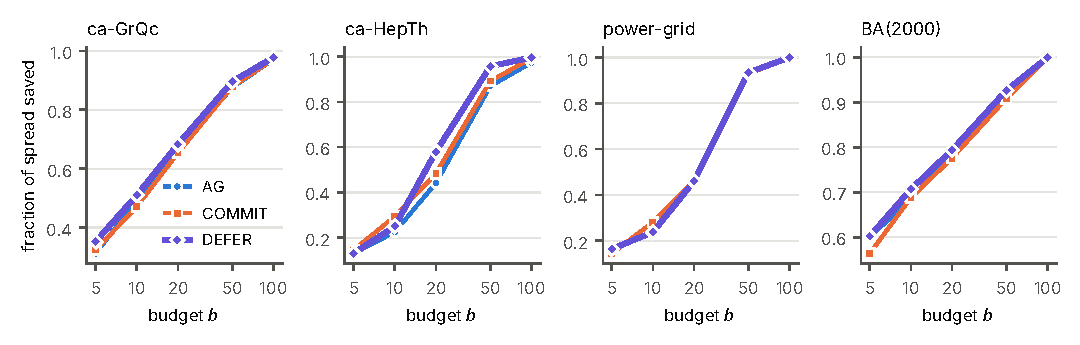
\includegraphics[width=0.6\textwidth]{figures/defer_budget_sweep.pdf}
\caption{Fraction of no-intervention spread saved as a function of budget, ca-GrQc, constant-probability model.\label{fig:defer-sweep}. Each point averages the live-edge draws available at that budget (2--8 draws depending on budget; see \texttt{results/summary\_adaptive.csv}).}
\end{figure}

Table~\ref{tab:defer-allbudgets} extends this comparison to all four
networks and the full budget sweep $b\in\{5,10,20,50,100\}$ under the
constant-probability model, restricted to AG, DEFER, and COMMIT for
readability.

\begin{table}[h]
\centering
\caption{Fraction of no-intervention spread saved across the full budget sweep, constant probability\label{tab:defer-allbudgets}}
\begin{tabular}{@{}lcccccccccccc@{}}
\hline
\up & \multicolumn{3}{c}{ca-GrQc} & \multicolumn{3}{c}{ca-HepTh} & \multicolumn{3}{c}{power-grid} & \multicolumn{3}{c}{BA(2000)} \\
$b$ & AG & DEFER & COMMIT & AG & DEFER & COMMIT & AG & DEFER & COMMIT & AG & DEFER & COMMIT \\
\hline
\up 5 & 0.250 & \textbf{0.259} & 0.186 & 0.283 & \textbf{0.322} & 0.235 & \textbf{0.130} & 0.124 & 0.053 & 0.463 & \textbf{0.463} & 0.419 \\
10 & 0.407 & \textbf{0.422} & 0.389 & 0.331 & \textbf{0.352} & 0.345 & \textbf{0.216} & \textbf{0.216} & 0.188 & 0.521 & \textbf{0.522} & 0.513 \\
20 & 0.583 & \textbf{0.602} & 0.591 & 0.452 & \textbf{0.471} & 0.448 & 0.339 & \textbf{0.341} & 0.290 & 0.571 & \textbf{0.573} & 0.562 \\
50 & 0.815 & \textbf{0.818} & 0.801 & 0.656 & \textbf{0.666} & 0.631 & \textbf{0.592} & \textbf{0.592} & 0.583 & 0.671 & 0.673 & \textbf{0.674} \\
\down 100 & \textbf{0.900} & \textbf{0.900} & 0.897 & 0.671 & 0.679 & \textbf{0.727}$^{*}$ & \textbf{0.788} & \textbf{0.788} & 0.785 & \textbf{0.795} & \textbf{0.795} & 0.767 \\
\hline
\end{tabular}
{\footnotesize Bold marks the best of the three policies shown per cell (ties bolded on
both). $^{*}$The one cell where COMMIT beats both AG and DEFER
(ca-HepTh, $b=100$) has only two live-edge draws, the smallest sample in
the sweep; we read it as more likely to be sampling noise than a real
reversal, but this is a judgment call, not something the two draws can
establish -- see \texttt{results/summary\_adaptive.csv} for the per-cell
standard errors omitted from the table for space. DEFER is at least tied
with AG in 19 of 20 cells and strictly ahead in 14, a tally that treats
every cell as equally informative regardless of its draw count (2--8 draws
depending on budget and network); the narrowing-at-large-budget pattern of
Figure~\ref{fig:defer-sweep} is nonetheless visible on every network.}
\end{table}

Two further robustness checks are reported in
Appendix~\ref{ec:seed-sensitivity}: a single-draw sweep with 50
highest-degree seeds (a harder, more concentrated seeding), where the
qualitative ranking DEFER $\ge$ AG still holds in 10 of 12 cells; and
\texttt{isocut}/\texttt{defer\_cut}, two constructions of our own
(Theorem~\ref{thm:isocut-separation}'s worst-case separation does not
materialize on these real networks, where \texttt{isocut} is
statistically indistinguishable from AG).
\subsection{Exact scenario-based integer-programming baselines}\label{sec:exp-ilp}

\paragraph{Formulation.} At a decision point the controller samples $K$
live-edge scenarios of the unobserved part of the cascade (edges out of the
frontier and out of inactive nodes; edges out of earlier active nodes have
already been tested and are dead) and solves the time-indexed sample-average
program
\[
\min \tfrac1K\sum_k\sum_v z_{kvD_k}\quad\text{s.t.}\quad
z_{kvd}\ge z_{ku,d-1}-\sum_{t<d}b_{kvt},\;\; z_{kvd}\ge z_{kv,d-1},\;\;
\sum_{v,t}b_{kvt}\le r,
\]
where $z_{kvd}$ indicates that $v$ is active by step $d$ in scenario $k$,
$b_{kvt}$ blocks $v$ before step $t$, and $r$ is the remaining budget. The
horizon $D_k$ is the unblocked cascade depth plus a slack of 4 steps, capped at
the number of reachable nodes (blocking can delay arrivals beyond the unblocked
depth, so the cap is the exact horizon and the slack is a truncation). With
the slack set to the cap, the one-shot model matches exhaustive search over all
blocking sets on the same scenarios (\texttt{tests/test\_ilp.py}, budgets
$1$--$3$). The models are solved with HiGHS (via SciPy) with a 30-second limit per
solve and relative gap $10^{-4}$. Two controllers use it.
\texttt{ilp1} is the one-shot optimum for the sampled scenarios, solved at time
$0$ with the whole budget (the exact counterpart of AG/GR).
\texttt{ilp\_roll} is a rolling-horizon staged model with $K=48$ scenarios in
$12$ first-step branches: blocks now are shared by all scenarios, blocks after
the first step are shared within a branch (non-anticipativity), and blocks at
step $2$ are scenario-specific recourse, which is optimistic. Only the blocks
now are committed, after which the controller observes and re-solves.

\paragraph{ILP inside DEFER.} Table~\ref{tab:defer-ilp} reports the same
instances and realizations with the one-shot ILP used as DEFER's planner. The
ILP's round-0 solution is the initial plan (as for the other wrapped planners),
re-planning solves the ILP on DEFER's own samples (first 48, 10-second limit),
and plan protection and push-down are unchanged. \texttt{COMMIT-ILP} re-solves
every round and commits the whole plan. The solver time limit makes the
highschool2013 rows depend on machine load.

\begin{table}[h]
\centering
\caption{Saved fraction of spread with the ILP as the one-shot planner inside DEFER,
and time per episode of \texttt{DEFER-ILP} (seconds).\label{tab:defer-ilp}}
\footnotesize
\begin{tabular}{lrrrrrrrr}
\hline
Network & $p$ & $b$ & DEFER & ilp1 & DEFER-ILP & nopush & COMMIT-ILP & t(DEFER-ILP)\\
\hline
dolphin & 0.1 & 2 & 0.250 & 0.319 & 0.325 & 0.319 & 0.188 & 0.04 \\
dolphin & 0.1 & 4 & 0.469 & 0.412 & 0.419 & 0.412 & 0.431 & 0.04 \\
dolphin & 0.1 & 8 & 0.744 & 0.756 & 0.762 & 0.756 & 0.706 & 0.03 \\
dolphin & 0.2 & 2 & 0.428 & 0.438 & 0.447 & 0.447 & 0.382 & 0.88 \\
dolphin & 0.2 & 4 & 0.570 & 0.570 & 0.567 & 0.572 & 0.588 & 0.78 \\
dolphin & 0.2 & 8 & 0.852 & 0.843 & 0.817 & 0.843 & 0.812 & 0.54 \\
iceland & 0.3 & 2 & 0.752 & 0.765 & 0.765 & 0.765 & 0.716 & 0.56 \\
iceland & 0.3 & 4 & 0.945 & 0.946 & 0.945 & 0.946 & 0.923 & 0.24 \\
iceland & 0.3 & 8 & 0.976 & 0.976 & 0.973 & 0.976 & 0.955 & 0.18 \\
karate & 0.2 & 2 & 0.602 & 0.590 & 0.596 & 0.596 & 0.607 & 0.11 \\
karate & 0.2 & 4 & 0.802 & 0.805 & 0.791 & 0.811 & 0.833 & 0.09 \\
workplace & 0.05 & 2 & 0.268 & 0.256 & 0.256 & 0.256 & 0.275 & 0.30 \\
workplace & 0.05 & 4 & 0.428 & 0.398 & 0.409 & 0.400 & 0.480 & 0.31 \\
workplace & 0.05 & 8 & 0.524 & 0.526 & 0.553 & 0.526 & 0.579 & 0.32 \\
BA-150 & 0.1 & 2 & 0.456 & 0.412 & 0.412 & 0.412 & 0.485 & 0.04 \\
BA-150 & 0.1 & 4 & 0.574 & 0.574 & 0.574 & 0.574 & 0.662 & 0.04 \\
BA-150 & 0.1 & 8 & 0.757 & 0.772 & 0.757 & 0.772 & 0.750 & 0.03 \\
highschool2013 & 0.03 & 4 & 0.214 & 0.181 & 0.149 & 0.149 & 0.172 & 25.36 \\
highschool2013 & 0.03 & 8 & 0.440 & 0.359 & 0.397 & 0.355 & 0.326 & 27.64 \\
\hline
\end{tabular}
\end{table}

\paragraph{Results.} Table~\ref{tab:ilp} gives the saved fraction of spread on
the same realizations used for every other policy (10 seed sets $\times$ 5
realizations per cell). Differences between policies are mostly within $0.03$
of saved fraction, and standard errors of the underlying spreads are large
relative to them (for example, $4.9$--$7.0$ on highschool2013); we did not run
paired significance tests. Counting cells where saved fractions differ by more than $0.02$:
\texttt{ilp1} is above AG in 1 of 19 cells and below it in 5; \texttt{ilp\_roll}
is above DEFER in 3 of 19 and below in 12; \texttt{COMMIT} is above DEFER in 11
and below in 2. On highschool2013, 47 of 100 \texttt{ilp1} solves and 26 of 971
\texttt{ilp\_roll} solves reached the time limit and returned the incumbent, and
the ILP controllers are well below the greedy ones (budget $8$: $0.312$ and
$0.162$ against $0.425$ for AG). The ILP controllers also cost orders of
magnitude more time per episode.

\begin{table}[h]
\centering
\caption{Saved fraction of spread and time per episode (seconds): greedy and DEFER
policies against the scenario-based ILP controllers. Constant edge probability
$p$; same realizations for all policies.\label{tab:ilp}}
\footnotesize
\begin{tabular}{lrrrrrrrrrr}
\hline
Network & $p$ & $b$ & AG & DEFER & COMMIT & ilp1 & ilp\_roll & t(AG) & t(ilp1) & t(roll)\\
\hline
dolphin & 0.1 & 2 & 0.269 & 0.250 & 0.344 & 0.319 & 0.281 & 0.00 & 0.03 & 0.12 \\
dolphin & 0.1 & 4 & 0.469 & 0.469 & 0.500 & 0.412 & 0.512 & 0.00 & 0.03 & 0.11 \\
dolphin & 0.1 & 8 & 0.744 & 0.744 & 0.781 & 0.756 & 0.738 & 0.00 & 0.02 & 0.07 \\
dolphin & 0.2 & 2 & 0.430 & 0.428 & 0.427 & 0.438 & 0.175 & 0.00 & 0.69 & 4.03 \\
dolphin & 0.2 & 4 & 0.573 & 0.570 & 0.617 & 0.570 & 0.423 & 0.00 & 0.65 & 8.76 \\
dolphin & 0.2 & 8 & 0.855 & 0.852 & 0.820 & 0.843 & 0.763 & 0.00 & 0.45 & 3.24 \\
iceland & 0.3 & 2 & 0.752 & 0.752 & 0.809 & 0.765 & 0.720 & 0.00 & 0.43 & 4.43 \\
iceland & 0.3 & 4 & 0.946 & 0.945 & 0.938 & 0.946 & 0.920 & 0.00 & 0.20 & 0.55 \\
iceland & 0.3 & 8 & 0.978 & 0.976 & 0.974 & 0.976 & 0.964 & 0.00 & 0.14 & 0.27 \\
karate & 0.2 & 2 & 0.596 & 0.602 & 0.599 & 0.590 & 0.551 & 0.00 & 0.09 & 0.70 \\
karate & 0.2 & 4 & 0.816 & 0.802 & 0.833 & 0.805 & 0.831 & 0.00 & 0.07 & 0.14 \\
workplace & 0.05 & 2 & 0.268 & 0.268 & 0.321 & 0.256 & 0.027 & 0.00 & 0.22 & 1.19 \\
workplace & 0.05 & 4 & 0.430 & 0.428 & 0.434 & 0.398 & 0.203 & 0.00 & 0.20 & 2.41 \\
workplace & 0.05 & 8 & 0.535 & 0.524 & 0.577 & 0.526 & 0.428 & 0.00 & 0.20 & 2.29 \\
BA-150 & 0.1 & 2 & 0.471 & 0.456 & 0.507 & 0.412 & 0.441 & 0.00 & 0.03 & 0.08 \\
BA-150 & 0.1 & 4 & 0.566 & 0.574 & 0.632 & 0.574 & 0.566 & 0.00 & 0.03 & 0.07 \\
BA-150 & 0.1 & 8 & 0.757 & 0.757 & 0.721 & 0.772 & 0.662 & 0.00 & 0.03 & 0.15 \\
highschool2013 & 0.03 & 4 & 0.212 & 0.214 & 0.264 & 0.183 & 0.072 & 0.01 & 19.36 & 52.03 \\
highschool2013 & 0.03 & 8 & 0.425 & 0.440 & 0.434 & 0.312 & 0.162 & 0.01 & 21.96 & 50.35 \\
\hline
\end{tabular}
\end{table}


\subsection{Computational cost}\label{sec:complexity-comparison}

Theorem~\ref{thm:defer-complexity} states DEFER's cost as AdvancedGreedy's per-round cost multiplied by the number of rounds $r$: adaptivity is not free computationally, even though pure deferral is free in expected spread (Theorem~\ref{thm:defer-dominates}). Measured wall-clock time per episode (Appendix Table~\ref{tab:timing}) confirms the shape: AG is cheapest on every network, GR is a small constant factor above it (about $1.1$--$1.3\times$), and DEFER and COMMIT are several times to an order of magnitude above both; DEFER/AG ranges from about $2.5\times$ on power-grid and BA(2000) to $4$--$7\times$ on ca-HepTh and ca-GrQc. COMMIT, not DEFER, is the most expensive throughout: its worse plan quality leaves the cascade active longer and adds re-planning rounds (Appendix~\ref{sec:complexity-practice}). The ILP controllers cost orders of magnitude more per episode (Section~\ref{sec:exp-ilp}).

\section{Discussion and Limitations}\label{sec:discussion}
\subsection{When does DEFER help in practice, and when is it unnecessary?}

Theorem~\ref{thm:adaptivity-gap} and Section~\ref{sec:defer-example}
locate the source of \texttt{DEFER-nopush}'s advantage precisely: it is
large when a vertex's protection is cheap to buy \emph{after} it is known
threatened but expensive \emph{unconditionally}, i.e.\ when activation
probabilities are low relative to the graph's branching factor. The
benchmark confirms this rather than merely asserting it: at budget $20$
under the constant-probability model, DEFER saves $0.2$--$1.9$ percentage
points more spread than AG on the four SNAP networks
(Table~\ref{tab:defer-results}), a margin that shrinks as the budget grows
(Figure~\ref{fig:defer-sweep}, Table~\ref{tab:defer-allbudgets}) and is
somewhat larger at small budgets ($0.2$--$3.9$ points over
$b\in\{5,10,20,50,100\}$), at roughly $2.5$--$7\times$ AG's per-episode
compute (Table~\ref{tab:timing});
under weighted cascade the margin is within the residual selection-bias
risk of Remark~\ref{rem:winners-curse}, so the extra compute buys little
there. A practitioner should ask whether the intervention has this shape
-- occasional high-fan-out gatekeepers, individually unlikely but
consequential -- rather than treat adaptivity as free and always better.
\texttt{DEFER-nopush} is never worse than its planner
(Theorem~\ref{thm:defer-dominates}); full DEFER is not
(Remark~\ref{rem:pushdown-counterexample}), though
Table~\ref{tab:defer-nopush-parity} in the the Appendix shows the two
agree to within $0.0075$ of saved fraction on every benchmark cell we ran.
DEFER also assumes full-adoption feedback with negligible latency: the
controller must observe each round's activations before the next round's
propagation, realistic when suspensions or quarantines are fast relative
to the cascade's own timescale, but not otherwise; noisy, delayed, or
partially-observed feedback is open.

\subsection{Relation to exact scenario-based methods}\label{sec:discussion-exact}

Exact optimization methods for blocking, such as the Benders and bilevel
algorithms of \citet{taninmis2022,taninmis2024}, suggest a natural dynamic
baseline: a time-indexed sample-average integer program in which blocking
variables carry a time index so the budget can be spent at different steps
(Section~\ref{sec:exp-ilp}). We implemented this model directly with an
off-the-shelf solver rather than their decomposition algorithms, in a one-shot
form (\texttt{ilp1}) and a rolling-horizon staged form (\texttt{ilp\_roll}),
and ran both on six networks of 34 to 327 nodes with 2--3 seeds and budgets of
2--8. Three observations follow, each limited to these small instances.

First, solving the sampled problem exactly did not beat greedy selection in
this benchmark. \texttt{ilp1} was within $0.02$ of AG's saved fraction in 13
of 19 cells, above it in one and below it in five. This is consistent with an exact evaluation of greedy on 60 small instances in a companion paper on exact evaluation of influence minimization, which found greedy exactly optimal on 56 of them, and it adds that the sampled optimum is itself a noisy
estimate of the true optimum, so exactness on the sample need not translate
into better out-of-sample plans. Second, the staged controller did not
outperform DEFER either: \texttt{ilp\_roll} was above DEFER in 3 cells and
below in 12. Its scenario-specific recourse lets it plan to react to futures it
cannot observe, and the tree-structured non-anticipativity we imposed covers
only the first step, so we regard it as one reasonable staged formulation, not
as the best achievable one. Third, cost: the ILP controllers needed
$0.02$--$52$ s per episode against milliseconds for AG and DEFER, and on the
327-node network they frequently hit the 30-second limit and fell well behind
the greedy methods, so these formulations did not scale to the sizes where
DEFER is used.

Two further points limit what the comparison shows. On the star-of-paths family
of Theorem~\ref{thm:adaptivity-gap} (Section~\ref{sec:exp-sop}), DEFER
saves $0.36$--$0.97$ of spread and exceeds the best of AG, GR, COMMIT and
\texttt{ilp1} in all 18 cells by at least $0.27$. A separate scan of larger
synthetic networks (Section~\ref{sec:exp-regime}) finds DEFER significantly
better than AG in 9 of 45 cells and worse in 0, with the gains in large-cascade regimes; the
small-instance cells above are mostly outside that regime. COMMIT, the
re-plan-and-commit-everything ablation, was above DEFER in 11 cells and below
in 2 in this small-instance regime, so on these instances the advantage of
deferral that Section~\ref{sec:defer-example} predicts for low-probability,
high-fan-out structure did not show up; the benchmark does not contradict
Theorem~\ref{thm:adaptivity-gap}, which is a worst-case statement, but it
does not support a practical advantage of deferral at these sizes either. We
also ran the ILP as the one-shot planner inside DEFER
(\texttt{DEFER-ILP}, Table~\ref{tab:defer-ilp}). Wrapping the
ILP in DEFER changed little: \texttt{DEFER-ILP} was within $0.02$ of
\texttt{ilp1} in 15 of 19 cells, and \texttt{DEFER-ILP} without push-down
within $0.02$ of \texttt{DEFER-ILP} in 16. It was below DEFER wrapped around AG in 5
cells and above in 2, and below COMMIT in 11 cells (above in 1). Committing the
ILP's plan every round (\texttt{COMMIT-ILP}) was the least stable variant,
and on highschool2013 80 of its 102 solves hit the time limit. These
comparisons share the caveats above, plus one more: a solve that hits the
wall-clock limit returns an incumbent that depends on machine load, so the
highschool2013 ILP numbers are not exactly reproducible (\texttt{ilp1} at
budget $8$ scored $0.312$ in one run and $0.359$ in the repeat). Staged exact formulations with larger scenario trees, decomposition methods, or
instances with the star-of-paths structure remain to be evaluated.

\subsection{Limitations}\label{sec:conclusion}

The evidence has four limits. First, the large synthetic scan and the empirical networks use constant or weighted-cascade edge probabilities and uniformly random or highest-degree seeds; the scan grid was chosen after seeing the small-instance results, so it is exploratory. Second, the SNAP-scale benchmark has few realizations per cell. Third, the star-of-paths family is constructed to have the structure the theory predicts, so it shows that the algorithm realizes the effect, not how common such structure is. Fourth, DEFER assumes full-adoption feedback with negligible latency; noisy, delayed or partially observed feedback is open. We did not implement the Benders and bilevel algorithms cited in Section~\ref{sec:related}.

\textbf{Code and data availability.} DEFER, the baselines and every benchmark script are released at \url{https://github.com/vinhqdang/trace_e}. Networks are generated by the released code (Barab\'asi--Albert, Erd\H{o}s--R\'enyi, tree, grid, geometric, Watts--Strogatz) or are the public datasets cited in Section~\ref{sec:defer-experiments}; the raw per-instance logs are in the same repository.

\begin{thebibliography}{99}
\providecommand{\natexlab}[1]{#1}
\providecommand{\url}[1]{\texttt{#1}}
\providecommand{\urlprefix}{URL }

\bibitem[{Asadpour and Nazerzadeh(2016)}]{asadpournazerzadeh2016}
Asadpour A, Nazerzadeh H (2016) Maximizing stochastic monotone submodular
  functions. \emph{Management Sci.} 62(8):2374--2391.

\bibitem[{Barab\'asi and Albert(1999)}]{barabasi1999}
Barab\'asi AL, Albert R (1999) Emergence of scaling in random networks.
  \emph{Science} 286(5439):509--512.

\bibitem[{Budak et~al.(2011)Budak, Agrawal, and El~Abbadi}]{budak2011}
Budak C, Agrawal D, El~Abbadi A (2011) Limiting the spread of misinformation
  in social networks. \emph{Proc.\ 20th Internat.\ Conf.\ on World Wide Web
  (WWW)}, 665--674.

\bibitem[{Dean et~al.(2008)Dean, Goemans, and Vondr\'ak}]{deangoemansvondrak2008}
Dean BC, Goemans MX, Vondr\'ak J (2008) Approximating the stochastic
  knapsack problem: The benefit of adaptivity. \emph{Math.\ Oper.\ Res.}
  33(4):945--964.

\bibitem[{Fan et~al.(2013)}]{fan2013}
Fan L, Lu Z, Wu W, Thuraisingham B, Ma H, Bi Y (2013) Least cost rumor
  blocking in social networks. \emph{Proc.\ 33rd IEEE Internat.\ Conf.\ on
  Distributed Computing Systems (ICDCS)}, 540--549.

\bibitem[{Farajtabar et~al.(2017)}]{farajtabar2017}
Farajtabar M, Yang J, Ye X, Xu H, Trivedi R, Khalil E, Li S, Song L, Zha H
  (2017) Fake news mitigation via point process based intervention.
  \emph{Proc.\ 34th Internat.\ Conf.\ on Machine Learning (ICML)},
  1097--1106.

\bibitem[{Golovin and Krause(2011)}]{golovinkrause2011}
Golovin D, Krause A (2011) Adaptive submodularity: Theory and applications
  in active learning and stochastic optimization. \emph{J.\ Artificial
  Intelligence Res.} 42:427--486.

\bibitem[{He et~al.(2012)}]{he2012}
He X, Song G, Chen W, Jiang Q (2012) Influence blocking maximization in
  social networks under the competitive linear threshold model.
  \emph{Proc.\ 2012 SIAM Internat.\ Conf.\ on Data Mining (SDM)}, 463--474.

\bibitem[{Kempe et~al.(2003)Kempe, Kleinberg, and Tardos}]{kempe2003}
Kempe D, Kleinberg J, Tardos {\'E} (2003) Maximizing the spread of influence
  through a social network. \emph{Proc.\ 9th ACM SIGKDD Internat.\ Conf.\ on
  Knowledge Discovery and Data Mining (KDD)}, 137--146.

\bibitem[{Leskovec et~al.(2007)}]{leskovec2007}
Leskovec J, Kleinberg J, Faloutsos C (2007) Graph evolution: Densification
  and shrinking diameters. \emph{ACM Trans.\ Knowledge Discovery from
  Data} 1(1):2.

\bibitem[{Lokhov et~al.(2014)}]{lokhov2014}
Lokhov AY, M\'ezard M, Ohta H, Zdeborov\'a L (2014) Inferring the origin
  of an epidemic with a dynamic message-passing algorithm. \emph{Phys.\
  Rev.\ E} 90:012801.

\bibitem[{Nguyen et~al.(2012)}]{nguyen2012}
Nguyen NP, Yan G, Thai MT, Eidenbenz S (2012) Containment of misinformation
  spread in online social networks. \emph{Proc.\ 4th Annual ACM Web Sci.\
  Conf.\ (WebSci)}, 213--222.

\bibitem[{Seeman and Singer(2013)}]{seemansinger2013}
Seeman L, Singer Y (2013) Adaptive seeding in social networks.
  \emph{Proc.\ 54th Annual IEEE Sympos.\ on Foundations of Computer Sci.\
  (FOCS)}, 459--468.

\bibitem[{Tan{\i}nm{\i}{\c s} et~al.(2022)}]{taninmis2022}
Tan{\i}nm{\i}{\c s} et al.\ (2022) Improved $x$-space algorithm for min-max
  bilevel problems with an application to misinformation spread in social
  networks. \emph{Eur.\ J.\ Oper.\ Res.} 297(1):40--52.

\bibitem[{Tan{\i}nm{\i}{\c s} et~al.(2024)}]{taninmis2024}
Tan{\i}nm{\i}{\c s} et al.\ (2024) Benders decomposition algorithms for
  minimizing the spread of harmful contagions in networks. \emph{Comput.\
  Oper.\ Res.} 167.

\bibitem[{Tong et~al.(2017)}]{tong2017}
Tong G, Wu W, Tang S, Du DZ (2017) Adaptive influence maximization in
  dynamic social networks. \emph{IEEE/ACM Trans.\ Networking} 25(1):112--125.

\bibitem[{Tong et~al.(2018)}]{tong2018}
Tong G, Wu W, Du DZ (2018) Distributed rumor blocking with multiple
  positive cascades. \emph{IEEE Trans.\ Comput.\ Social Systems} 5(2):468--480.

\bibitem[{Wang et~al.(2013)Wang, Zhao, Chen, Li, Zhang, and Xia}]{wang2013blocking}
Wang S, Zhao X, Chen Y, Li Z, Zhang K, Xia J (2013) Negative influence
  minimizing by blocking nodes in social networks. \emph{Late-Breaking
  Developments in the Field of Artificial Intelligence, Papers Presented at
  the 27th AAAI Conf.\ on Artificial Intelligence}, AAAI Technical Report
  WS-13-17, 134--136.

\bibitem[{Wang et~al.(2016)}]{wang2016drimux}
Wang B, Chen G, Fu L, Song L, Wang X (2016) DRIMUX: Dynamic rumor influence
  minimization with user experience in social networks. \emph{Proc.\ 30th
  AAAI Conf.\ on Artificial Intelligence (AAAI)}, 791--797.

\bibitem[{Wang et~al.(2024)Wang, Wu, Wang, Zhang, Qin, Zhang, and Lin}]{wang2024sandwich}
Wang J, Wu Y, Wang X, Zhang Y, Qin L, Zhang W, Lin X (2024) Efficient
  influence minimization via node blocking. \emph{Proc.\ VLDB Endowment}
  17(10):2501--2513.

\bibitem[{Watts and Strogatz(1998)}]{watts1998}
Watts DJ, Strogatz SH (1998) Collective dynamics of `small-world'
  networks. \emph{Nature} 393:440--442.

\bibitem[{Xiang et~al.(2024)Xiang, Wang, Wu, Wang, Chen, and Zhang}]{xiang2024}
Xiang F, Wang J, Wu Y, Wang X, Chen C, Zhang Y (2024) Rumor blocking with
  pertinence set in large graphs. \emph{World Wide Web} 27(1):Article 6.

\bibitem[{Xie et~al.(2023)Xie, Zhang, Wang, Lin, and Zhang}]{xie2023}
Xie J, Zhang F, Wang K, Lin X, Zhang W (2023) Minimizing the influence of
  misinformation via vertex blocking. \emph{Proc.\ 39th IEEE Internat.\
  Conf.\ on Data Engineering (ICDE)}, 3096--3108.

\bibitem[{Xie et~al.(2024)Xie, Zhang, Wang, Liu, Lin, and Zhang}]{xie2024}
Xie J, Zhang F, Wang K, Liu J, Lin X, Zhang W (2024) Influence minimization
  via blocking strategies. \emph{INFORMS J.\ Comput.}, forthcoming. Code:
  \texttt{github.com/INFORMSJoC/2024.0591}, arXiv:2312.17488.

\bibitem[{Yan et~al.(2020)}]{yan2020}
Yan R, Li D, Wu W, Du DZ, Wang Y (2020) Minimizing influence of rumors by
  blockers on social networks: Algorithms and analysis. \emph{IEEE Trans.\
  Network Science and Engineering} 7(3):1067--1078.

\bibitem[{Zareie and Sakellariou(2021)}]{zareie2021}
Zareie A, Sakellariou R (2021) Minimizing the spread of misinformation in
  online social networks: A survey. \emph{J.\ Network and Computer
  Applications} 186:103094.

\end{thebibliography}

\appendix
\section{Proofs for Section~\ref{sec:defer}}\label{ec:defer-proofs}

\begin{repeatlemma}[Lemma~\ref{lem:defer-free} (Deferral is free)]
Fix a live-edge realization, the seeds, and any set $P$ with $|P|\le b$. Let
$\pi_P$ be the policy that, in every round, blocks the not-yet-blocked
vertices of $P$ that are exposed to the current frontier. Then $\pi_P$
produces exactly the same final active set as blocking $P$ at time $0$, and
blocks at most as many vertices.
\end{repeatlemma}
\begin{proof}
On a fixed realization a vertex $v$ becomes active in the first round in
which a frontier vertex has a live edge into it, i.e.\ the round after it is
first exposed. $\pi_P$ blocks $v\in P$ in that round, before its trial, so
$v$ never activates; every vertex outside $P$ faces the same set of blocked
vertices at each of its trials under both policies, because a vertex of $P$
that is never exposed never takes part in any trial. Hence the activation
sequences coincide. Vertices of $P$ that are never exposed are never
blocked.
\end{proof}

\begin{repeattheorem}[Theorem~\ref{thm:defer-dominates} (\texttt{DEFER-nopush} weakly dominates its planner)]
Let $P_0$ be the plan of $\mathcal P$ at round $0$, and consider
Algorithm~\ref{alg:defer} with the push-down step removed
(\texttt{DEFER-nopush}: every exposed planned vertex is committed
immediately). If, in every later round, the plan-protection test only ever
replaces the leftover $L=P_{t-1}\setminus C_{t-1}$ by a new plan $P'$
whose held-out sample-average saving exceeds $L$'s by more than one
held-out standard error, then the expected final spread of
\texttt{DEFER-nopush} is at most that of the one-shot solution $P_0$, up to
the residual error of that one-sided test (Remark~\ref{rem:winners-curse}).
\end{repeattheorem}
\begin{proof}
By Lemma~\ref{lem:defer-free} the policy that keeps $P_0$ and commits
lazily (blocking every not-yet-blocked vertex of $P_0$ the moment it is
exposed) has the same spread as blocking $P_0$ at time $0$.
\texttt{DEFER-nopush} differs from it only by replacing, at each round,
the uncommitted leftover by a plan that clears the plan-protection test
for the remaining budget, and then committing \emph{every} exposed vertex
of the resulting plan immediately (no push-down deferral); the committed
prefix is otherwise identical to lazily committing whichever plan is
currently standing. If every swap were only ever made when $P'$ is truly
at least as good as $L$, induction over rounds would give the claim
exactly, since replacing a standing plan by an at-least-as-good one and
then committing lazily can only weakly improve on committing the original
lazily (again by Lemma~\ref{lem:defer-free}, applied to whichever plan is
current at each round). The test instead accepts $P'$ whenever its
held-out sample-average saving exceeds $L$'s by more than one held-out
standard error -- a one-sided test against equally-good alternatives,
using concentration of the sample average (\citealp{xie2024}, applied per
candidate plan) on data disjoint from whatever $P'$ was optimized on, so
the comparison itself is not confounded by having been optimized and
tested on the same draws. This rules out the most severe form of
optimizer's-curse bias (comparing a plan against the very data used to
select it) but not the residual chance that a $P'$ that is not truly
better than $L$ still clears the $1$-SE margin on a given round's held-out
draw; Remark~\ref{rem:winners-curse} discusses this residual, which we do
not bound here. Push-down is excluded from this argument entirely: it can
permanently forfeit protection of a deferred vertex if the budget that was
supposed to remain available for it is spent elsewhere first, which is
exactly the failure mode Remark~\ref{rem:pushdown-counterexample}
exhibits.
\end{proof}

\begin{repeatremark}[Remark~\ref{rem:winners-curse} (The 1-SE margin bounds, but does not eliminate, selection bias)]
Choosing between two noisy sample averages is a textbook source of
upward-biased apparent improvement (the ``winner's curse''): if $L$ and
$P'$ were in fact equally good, the test still swaps to $P'$ whenever its
held-out average happens to exceed $L$'s by more than one standard error,
which is not a negligible event. Requiring a fresh, held-out draw for the
comparison removes the optimistic bias of optimizing and testing on the
same data, and the $1$-standard-error margin makes an accidental swap less
likely than a bare $\arg\max$ would; neither removes the residual chance
that a truly worse plan clears the margin on a given round's held-out
draw. We do not prove a bound on the resulting regret here.
\end{repeatremark}

\begin{repeatlemma}[Lemma~\ref{lem:pushdown} (Push-down is the local myopic optimum)]
Consider an exposed planned vertex $v$ whose children (its inactive
out-neighbors) jointly protect the same set as $v$ minus $v$ itself, assume
the children are exposed only through $v$, and value a budget unit at
$\lambda$ vertices. Among the two policies ``block $v$ now'' and ``block
$v$'s children if and only if $v$ activates,'' the second has smaller
expected loss (vertices lost plus $\lambda$ times budget spent) if and only
if $q_v(c_v+1/\lambda)<1$.
\end{repeatlemma}
\begin{proof}
Blocking now costs $\lambda$ and loses nothing of $v$'s set. Waiting loses
$v$ (one vertex) and spends $c_v$ units with probability $q_v$, and nothing
otherwise, while the protected set is the same in both branches by
assumption: expected loss $q_v+\lambda q_v c_v$. Comparing $\lambda$ against
$q_v+\lambda q_v c_v$ gives the stated condition. Note that $\lambda$ is
treated as a fixed price at which a budget unit can always be redeployed;
the lemma says nothing about what happens when several vertices are
deferred under this reasoning simultaneously and the budget they were all
counting on cannot cover all of them at once
(Remark~\ref{rem:pushdown-counterexample}).
\end{proof}

\begin{repeatremark}[Remark~\ref{rem:pushdown-counterexample} (Push-down does not preserve domination)]
On the star-of-paths instance with $\Delta=2$, $p=0.4$, $L=1$, $b=1$
(Section~\ref{sec:defer-example}, Remark~\ref{rem:pushdown-counterexample}
give the setup and the headline numbers, $0.96$ vs.\ $0.8$), the
case-by-case detail behind that expected spread is: with
$k\sim\mathrm{Binomial}(2,p)$ gateways active, $k\le1$ contributes spread
$k$ (the one active branch, if any, is sealed at the cost of the vertex
already reached), while $k=2$ (probability $p^2=0.16$) leaves only one
budget unit for two simultaneously-deferred children, so one branch's
path vertex activates unblocked, contributing spread $2+L=3$. Summing,
$\Pr[k{=}0]\cdot0+\Pr[k{=}1]\cdot1+\Pr[k{=}2]\cdot3=0.36(0)+0.48(1)+0.16(3)=0.96$.
\end{repeatremark}

\begin{repeattheorem}[Theorem~\ref{thm:adaptivity-gap} (The adaptivity gap of IMIN is unbounded)]
For every $\Delta\ge 2$, $p\in(0,1)$, and path length $L\ge1$ there is an
instance with maximum out-degree $\Delta$, budget $1$, on which the best
one-shot solution and DEFER have expected savings $p(L+1)$ and
$L(1-(1-p)^\Delta)$ respectively, so DEFER's saving is
$\frac{L}{L+1}\cdot\frac{1-(1-p)^\Delta}{p}$ times the one-shot saving, a
factor tending to $(1-(1-p)^\Delta)/p$ (which itself tends to $\Delta$ as
$p\to0$) as $L\to\infty$; the ratio of the two policies' expected spreads
is, at every finite $L$, strictly \emph{less} than
$\frac{(\Delta-1)p}{\Delta p-1+(1-p)^\Delta}$, increasing to this value only
in the limit $L\to\infty$, which (taken before $p\to0$, for fixed $\Delta$)
diverges.
\end{repeattheorem}
\begin{proof}
Seed $s$ has out-neighbors $a_1,\dots,a_\Delta$ with $p(s,a_i)=p$; each
$a_i$ starts a private directed path of length $L$ with edge probability
$1$. Any one-shot solution with budget $1$ blocks one vertex; blocking
$a_i$ (or a vertex on its path) saves exactly $L+1$ vertices if $a_i$ is
activated, which happens with probability $p$, and nothing otherwise, so
its expected saving is $p(L+1)$ and its expected spread is
$(\Delta-1)p(L+1)$ (the other $\Delta-1$ branches are unprotected). DEFER
observes $N_1=\{a_i:(s,a_i)\text{ live}\}$ and blocks the first path vertex
of one activated branch (its plan at round $0$ is a branch head $a_i$ with
$q=p$, $c=1$, and $\lambda\approx pL$, so the push-down rule
$p(1+1/(pL))<1$ defers it); if $k$ branches are active the spread is
$(k-1)^+L+k$. Its expected saving is $L\Pr[k\ge1]=L(1-(1-p)^\Delta)$ (one
branch's continuation is sealed for the cost of the vertex already reached,
regardless of $k$) and its expected spread is
$\mathbb E[(k-1)^+]L+\Delta p=(\Delta p-1+(1-p)^\Delta)L+\Delta p$, using
$\mathbb E[(k-1)^+]=\mathbb E[k]-\Pr[k\ge1]=\Delta p-(1-(1-p)^\Delta)$.

Two distinct ratios follow from these exact expressions. The \emph{saving}
ratio is $\frac{L(1-(1-p)^\Delta)}{p(L+1)}=\frac{L}{L+1}\cdot
\frac{1-(1-p)^\Delta}{p}$, increasing in $L$ to the limit
$(1-(1-p)^\Delta)/p$, which tends to $\Delta$ as $p\to0$ (since
$1-(1-p)^\Delta=\Delta p-\binom\Delta2p^2+O(p^3)$). The \emph{spread} ratio
is $\frac{(\Delta-1)p(L+1)}{(\Delta p-1+(1-p)^\Delta)L+\Delta p}$. Writing
$A=(\Delta-1)p$, $B=\Delta p-1+(1-p)^\Delta$, $C=\Delta p$, this is
$A(L+1)/(BL+C)$, whose derivative with respect to $L$ has the sign of
$A(C-B)$; since $C-B=1-(1-p)^\Delta>0$, the ratio is strictly increasing in
$L$ for every finite $L\ge1$ and tends to its supremum $A/B=\frac{(\Delta-1)p}
{\Delta p-1+(1-p)^\Delta}$ only as $L\to\infty$ -- so at any finite $L$ the
spread ratio is strictly below this value, not at least it. Taking
$L\to\infty$ first (for fixed $\Delta,p$) and only then $p\to0$: the
denominator $B$ behaves like $\binom\Delta2p^2$ as $p\to0$ (the $O(p)$
terms cancel), so the $L\to\infty$ limit $A/B$ behaves like
$\frac{(\Delta-1)p}{\binom\Delta2p^2}=\frac{2}{\Delta p}\to\infty$ --
already unbounded at $\Delta=2$, independently of the saving ratio's
$\Delta\to\infty$ argument, but only once $L$ has been sent to infinity
first: for any \emph{fixed} $L$, the same ratio $A(L+1)/(BL+C)$ tends
instead to $A(L+1)/C=(\Delta-1)(L+1)/\Delta$ as $p\to0$ (since $B\to0$
faster than $C$), a finite constant, so the order of the two limits is not
interchangeable. The two ratios are genuinely different quantities -- the
savings' ratio bound does not apply to the spreads' ratio -- and both
statements above are established directly from the same exact closed
forms, with no approximation beyond the stated limits.
\end{proof}

\begin{repeattheorem}[Theorem~\ref{thm:defer-complexity} (Complexity of DEFER)]
Let $n_t,m_t$ be the number of vertices and edges reachable from $F_t$ in
the union of the $\theta$ samples, $r$ the number of rounds, and $\alpha$
the inverse Ackermann function. With the dominator planner, round $t$
costs $O(\theta\,m_t\,\alpha(m_t,n_t))$ for the dominator trees plus
$O(b_t\,\theta'\,m_t\,\alpha)$ for the greedy picks; the total is
$O\bigl(\sum_t(1+b_t)\,\theta\,m_t\,\alpha\bigr)$, which is
$O(r\,b\,\theta\,m\,\alpha(m,n))$ in the worst case.
\end{repeattheorem}
\begin{proof}
Each dominator tree is computed by the Cooper--Harvey--Kennedy iteration
on the reachable subgraph (near-linear; the Lengauer--Tarjan analysis gives
the $\alpha$ bound). Drawing $\theta$ live-edge samples reachable from
$F_t$ (Algorithm~\ref{alg:defer}) is a breadth-first search per sample. Recomputation after a pick is restricted to samples
whose cached reach set contains the picked vertex, which is exactly the
set of samples whose dominator tree can change. Summing over picks and
rounds gives the bound.
\end{proof}

\begin{repeattheorem}[Theorem~\ref{thm:isocut-separation} (Isolation-move separation)]
There is a family of instances on which AdvancedGreedy, GreedyReplace, and
the Sandwich lower-bound greedy all save $O(b)$ vertices with budget $b$,
while a planner with frontier-isolation moves saves $\Omega(N)$ for
arbitrary $N$.
\end{repeattheorem}
\begin{proof}
Construction: a decoy seed with $b+1$ out-neighbors, each with one private
leaf (single-vertex saving 2); a real seed with $c\le b$ out-neighbors, all
of which point to every vertex of a region $R$ of $N$ vertices whose
vertices have no private successors. Every single vertex in $R$ or among
the real seed's out-neighbors saves at most 1, so all three published
rules spend the budget on decoy neighbors (saving $2b$; GreedyReplace's
replacement pass replaces a decoy blocker by itself and stops), whereas
isolating the real seed saves $N+c$ at cost $c$.
\end{proof}

\section{Seed-Selection Sensitivity and Isolation-Move Ablations}\label{ec:seed-sensitivity}

\subsection{Seed-selection sensitivity}

The main-body results seed with 20 uniformly random vertices. We
additionally ran a single-draw sweep with 50 highest-degree seeds -- a
harder, more concentrated seeding -- across the same networks and budgets
$10,20,50$ (Table~\ref{tab:defer-degree-seeds}). These noisier (one draw
per cell) numbers still show DEFER weakly at or above AG in 10 of 12
cells; the two exceptions (ca-GrQc $b=10$, ca-HepTh $b=50$) are
single-draw, small-margin reversals of the kind
Remark~\ref{rem:winners-curse} anticipates, not evidence against
Theorem~\ref{thm:defer-dominates}. Power-grid $b=50$ is a tie, not a
reversal. High-degree seeding also compresses push-down's opportunity and
gives COMMIT less chance to lock in a bad early commitment, so COMMIT is
no longer uniformly dominated here (it is the single-draw winner on
several cells).

\begin{table}[h]
\centering
\caption{Fraction of spread saved, 50 highest-degree seeds, single draw per cell, constant probability\label{tab:defer-degree-seeds}}
\begin{tabular}{@{}lcccccccccccc@{}}
\hline
\up & \multicolumn{3}{c}{ca-GrQc} & \multicolumn{3}{c}{ca-HepTh} & \multicolumn{3}{c}{power-grid} & \multicolumn{3}{c}{BA(2000)} \\
$b$ & AG & DEFER & COMMIT & AG & DEFER & COMMIT & AG & DEFER & COMMIT & AG & DEFER & COMMIT \\
\hline
\up 10 & 0.317 & 0.314 & \textbf{0.325}$^\dagger$ & 0.121 & 0.121 & \textbf{0.122}$^\dagger$ & 0.148 & \textbf{0.153} & 0.146 & 0.340 & 0.342 & \textbf{0.344}$^\dagger$ \\
20 & 0.471 & 0.474 & \textbf{0.476}$^\dagger$ & 0.229 & 0.231 & \textbf{0.237}$^\dagger$ & 0.231 & \textbf{0.238} & 0.214 & 0.395 & \textbf{0.397} & 0.388 \\
\down 50 & 0.691 & 0.696 & \textbf{0.709}$^\dagger$ & \textbf{0.472} & 0.461 & 0.464 & 0.404 & 0.404 & \textbf{0.411}$^\dagger$ & 0.470 & 0.474 & \textbf{0.478}$^\dagger$ \\
\hline
\end{tabular}
{\footnotesize $^\dagger$Cells where the single-draw realization favors AG or COMMIT
over DEFER by a small margin; see the discussion in the text. Bold marks
the nominal best value per cell, which at $n=1$ draw is a point estimate
rather than a statistically distinguishable ranking.}
\end{table}

\subsection{Complexity in practice}\label{sec:complexity-practice}

The wall-clock measurements behind the main text's timing discussion
(Section~\ref{sec:complexity-comparison}): COMMIT, despite executing the
identical per-round algorithm as DEFER, costs \emph{more} than DEFER on
every network, because its inferior plan quality
(Tables~\ref{tab:defer-results}, \ref{tab:defer-allbudgets}) leaves the
cascade active longer, adding re-planning rounds.

\begin{table}[h]
\centering
\caption{Wall-clock time per episode (seconds), budget 20, constant probability\label{tab:timing}}
\begin{tabular}{@{}lccccc@{}}
\hline
\up network ($n$) & AG & GR & DEFER & COMMIT & isocut \\
\hline
\up ca-GrQc (5241) & 0.078 & 0.085 & 0.542 & 0.861 & 0.080 \\
ca-HepTh (9875) & 0.232 & 0.272 & 1.002 & 1.793 & 0.238 \\
power-grid (4941) & 0.006 & 0.008 & 0.017 & 0.048 & 0.010 \\
\down BA(2000) (2000) & 0.012 & 0.014 & 0.030 & 0.088 & 0.016 \\
\hline
\end{tabular}
{\footnotesize Isocut (a one-shot planner with the added frontier-isolation move of
Theorem~\ref{thm:isocut-separation}) costs about as much as AG, since it
adds one candidate-move type to a single planning call rather than
introducing DEFER's round-by-round re-planning.}
\end{table}

\subsection{Isolation moves in practice}\label{sec:isocut-practice}

\texttt{isocut} (AG extended with a frontier-isolation move) and
\texttt{defer\_cut} (DEFER wrapping \texttt{isocut}) are our own
constructions, not literature baselines. Theorem~\ref{thm:isocut-separation}
shows a worst-case family where isolation moves save $\Omega(N)$ against
every other rule's $O(b)$; Table~\ref{tab:isocut} checks whether this
shows up on the real SNAP-scale networks used throughout, and it does
not -- isocut is statistically indistinguishable from AG, and
defer\_cut is at best a marginal improvement (ca-HepTh) and a marginal
loss elsewhere. This reflects which graphs the adversarial construction's
decoy-seed structure resembles, not a failure of the proof: real
collaboration/infrastructure networks rarely have a seed whose entire
out-neighborhood points into an otherwise-unreachable region, so the move
is a documented worst-case possibility, not a default-algorithm
component.

\begin{table}[h]
\centering
\caption{Fraction of no-intervention spread saved, isolation-move ablations, budget 20, constant probability\label{tab:isocut}}
\begin{tabular}{@{}lcccc@{}}
\hline
\up network & AG & DEFER & isocut & defer\_cut \\
\hline
\up ca-GrQc & 0.583 & \textbf{0.602} & 0.574 & 0.589 \\
ca-HepTh & 0.452 & 0.471 & 0.452 & \textbf{0.488} \\
power-grid & 0.339 & \textbf{0.341} & 0.339 & \textbf{0.341} \\
\down BA(2000) & 0.571 & \textbf{0.573} & 0.571 & \textbf{0.573} \\
\hline
\end{tabular}
{\footnotesize Bold marks the best value per row. isocut never beats AG; defer\_cut
beats plain DEFER only on ca-HepTh and ties it elsewhere.}
\end{table}

\section{Experimental Protocol}\label{ec:reproducibility}
Graphs: ca-GrQc, ca-HepTh, a power-grid network, a Barab\'asi--Albert
random graph with 2000 vertices, and soc-Epinions1 where feasible.
Probabilities: constant $p\in\{0.05,0.1\}$ and the weighted-cascade model.
Seeds: 20 or 50, drawn uniformly at random or as the highest-degree
vertices. Budgets: 20, 50, 100. For each instance and each of 5 independent
live-edge realizations, every policy runs on the same realization with the
same total budget (common random numbers), so differences are attributable
to policy alone. Policies compared: none, AdvancedGreedy, GreedyReplace,
the Sandwich lower bound, proximity-to-seeds, degree (all one-shot); DEFER
with the dominator planner, DEFER with GreedyReplace as planner, COMMIT,
and DEFER restricted to a 4-round planning horizon. Reported: final spread
beyond the seeds (mean and standard error), fraction of spread saved,
budget used, and wall-clock time per episode including planning.

Table~\ref{tab:defer-nopush-parity} compares full DEFER and
\texttt{DEFER-nopush} directly on the same live-edge draws, at budget 20,
for every (network, probability model) cell in
Table~\ref{tab:defer-results}, independent of that table's own
aggregation.

\begin{table}[h]
\centering
\caption{Fraction of no-intervention spread saved, budget 20: full DEFER vs.\ \texttt{DEFER-nopush}\label{tab:defer-nopush-parity}}
\begin{tabular}{@{}lcccccccc@{}}
\hline
\up & \multicolumn{4}{c}{constant probability} & \multicolumn{4}{c}{weighted cascade} \\
policy & ca-GrQc & ca-HepTh & power-grid & BA(2000) & ca-GrQc & ca-HepTh & power-grid & BA(2000) \\
\hline
\up DEFER & 0.667 & 0.820 & 0.466 & 0.798 & 0.391 & 0.339 & 0.394 & 0.424 \\
\down \texttt{DEFER-nopush} & 0.666 & 0.820 & 0.466 & 0.798 & 0.391 & 0.339 & 0.394 & 0.424 \\
\hline
\end{tabular}
{\footnotesize Values differ from Table~\ref{tab:defer-results} because that table
pools across the two constant-probability settings $p\in\{0.05,0.1\}$,
while this table reports a single $p=0.1$ draw per network to keep the
two policies' inputs identical; see
\texttt{results/summary\_adaptive.csv}. Across all eight cells here, and
across every budget in $\{5,10,20,50,100\}$ on the same
20-random-seed runs, \texttt{DEFER-nopush} agrees with full DEFER to
within $0.0075$ of saved fraction, and is identical to three decimal
places in the large majority of cells -- push-down essentially never
changes the outcome on these benchmarks, even though
Remark~\ref{rem:pushdown-counterexample} shows it can in principle.}
\end{table}

\end{document}
